\documentclass[10pt,twocolumn,letterpaper]{article}

\usepackage{cvm}
\usepackage{times}
\usepackage{epsfig}
\usepackage{graphicx}
\usepackage{amsmath}
\usepackage{amssymb}

\usepackage{mathtools}

% Include other packages here, before hyperref.

% If you comment hyperref and then uncomment it, you should delete
% egpaper.aux before re-running latex.  (Or just hit 'q' on the first latex
% run, let it finish, and you should be clear).
\usepackage[pagebackref=true,breaklinks=true,letterpaper=true,colorlinks,bookmarks=false]{hyperref}

\cvmfinalcopy
% \cvmfinalcopy % *** Uncomment this line for the final submission

\def\cvmPaperID{****} % *** Enter the cvm Paper ID here
\def\httilde{\mbox{\tt\raisebox{-.5ex}{\symbol{126}}}}

% Pages are numbered in submission mode, and unnumbered in camera-ready
\ifcvmfinal\pagestyle{empty}\fi
\begin{document}

%%%%%%%%% TITLE
\title{Propagated Mesh Normal Filtering}

\author{First Author\\
Institution1\\
Institution1 address\\
{\tt\small firstauthor@i1.org}
% For a paper whose authors are all at the same institution,
% omit the following lines up until the closing ``}''.
% Additional authors and addresses can be added with ``\and'',
% just like the second author.
% To save space, use either the email address or home page, not both
\and
Second Author\\
Institution2\\
First line of institution2 address\\
{\small\url{http://www.author.org/~second}}
}

\maketitle
% \thispagestyle{empty}

\begin{abstract}
    The bilateral filter is a classical filtering operator with the goal of preserving edge structure while smoothing signals.
    The reason it works is mainly on the spatial and range distances are enough close, but it ignores the local connections between signals.
    In this paper, we introduce a intrinsic filter method for 2D manifold surfaces.
    This approach builds the connections between desired signal and its neighbors shown in figure~\ref{Fig:relation}.
    Therefore, it has a outstanding power on filtering neighbor signal while preserving the important feature.
    A novel filtering framework based on our intrinsic filter is proposed with application in mesh denoising.
    As the traditional mesh filtering, our framework also has two-stage process:
    first, we apply geodesic path to build the face normal connections, then filter the face normals basing two different accumulative distance weights.
    afterwards, the vertex positions are updated according to the filtered face normals.
    For accelerating this process, we also introduce a simple, fast and effective pattern to replace the expend of using geodesic path
    It performs well on a wide variety of meshes and is competitive with other state-of-the-art methods.

    %The Computational Visual Media Conference series, of which this is to be the first conference, is intended to provide a major new international forum for exchanging novel research ideas and significant %practical results both underpinning and applying Visual Media.
\end{abstract}



\section{Introduction}

Due to the popularity of 3D scanners, meshes are becoming more and more accessible.
However, the influence of environment and people makes the data contain a lot of high frequency noises.
Mesh filtering is a vital preprocessing tool of updating vertex positions in a mesh to achieve perfect goals like denoising, smoothing or enhancement.
It typically preserve the obvious geometric structures, while undesirable noise need be discarded.
Although a variety of mesh filtering methods achieve satisfactory results \cite{fleishman2003bilateral, zheng2011bilateral},
they have a little imperfect result in dealing with the geometry features such as edges and corners.
Because the characteristics of adjacent regions are blended, the output mesh would be imperfect.

The bilateral filter, introduced in \cite{tomasi1998bilateral}, is a famous edge-preserving image filter, which prefers near values to distant values in both domain and range.
Unlike this bilateral filter, the guided filters \cite{Petschnigg2004, he2010guided} set the filtering weights using the intensity difference from another image and has better edge-preserving property.
Due to their success in image processing and computational photography and considering normals as a surface signal defined over the original mesh,
many attempts have been made to adapt them to geometry processing such as mesh denoising and smoothing \cite{jones2003non, zheng2011bilateral, Solomon2014general}.
These filter are able to alleviate the smooth problem, but they still have disadvantages in the process of preserving image/mesh context.
For example, choosing a large neighborhood will result in blend of cross-region, while selecting a small one would limit the filtering performance.

Recently,  propagated image filter \cite{Chang2015propagated} was addressed and display its powerful filtering performance.
It calculates the accumulated difference not only between the values of adjacent pixels, but also start-end pixels in choosing shortest path.
Then it dynamically determines their filtering weight by these two accumulated difference.
As the accumulated difference has the ability to weigh the image context, the propagated filter has a more superior edge-preserving property.

In this paper, we successfully apply the propagated filtering to geometry processing.
Similar to the previous method, we consider normals as a surface signal defined over the original mesh because of its sensitivity to mesh feature.
We discard the shortest path algorithm in selecting filtered path because the time cost is expensive.
A simple and effective method is put forward for solving that problem.
For filtering the normal signal, we project its neighborhood onto a surface based on its normals.
Then the areal coordination is used to divide its neighbor to seven regions. To a certain extent, the seven regions depict the local characteristics of the mesh.
Afterwards, we sort its neighborhood though the difference of distance in same region.
Though above operations, a fixed pattern can be obtained and be used for selecting the filtered path.
Finally, we apply propagated filtering to the face normals, then update the mesh vertices to match the filtered face normals.
The effectiveness of our approach is illustrated by extensive experimental results in mesh denoising and smoothing.
\section{Relate work}

The rise of 3D scanning devices makes captured meshes become more and more easier.
However, as the influence of light or devices, meshes which are taken often contain high-frequency noises.
Thus mesh denoising, as an important tool of geometry processing, becomes a popular study point~\cite{Wang2008comprehensive}.
Due to the large amount of research work in this field, we introduce some methods that have similarities with ours.

The purpose of mesh denoising is removing the noise without damaging the true structure.
Because the edge-preserving property of bilateral filter~\cite{tomasi1998bilateral}, it is widely used in image processing~\cite{oh2001image, durand2002fast, Barash2004common, Wang2014decoupling} and geometry processing such as mesh denoising~\cite{fleishman2003bilateral, jones2003non, zheng2011bilateral, Solomon2014general} and mesh feature enhancement~\cite{Wang2006bilateral}.

The papers \cite{fleishman2003bilateral} and ~\cite{jones2003non} apply bilateral filter to the mesh vertex positions as it is used in image denoising~\cite{durand2002fast}.
\cite{zheng2011bilateral} employ the bilateral filter to the mesh face normals, then according the filtered normals the process of vertex updated is implemented.
\cite{Solomon2014general} also perform mesh denoising by filtering the face normals, using a generalized cross-bilateral filter.
The effectiveness of bilateral filter relies on the range function which reflects the local information of signal, and then applies the averaging weights as the filtered output.
However, the difference between the input signal values $J_{p}$ and $J_{q}$ can not provides reliable prediction for that between the desired signal values $\bar{J_{p}}$ and $\bar{J_{q}}$.
Our denoising algorithm also applies the similar approach which iterates face normal filtering and vertex updates.
However, our method differs from \cite{zheng2011bilateral} and \cite{Solomon2014general} which both only consider the spatial and range distances that may smooth the weak edges,
also is different from~\cite{Zhang2015Filter} which uses a joint bilateral filter on the normals that may break the sharp corners.
As we build the connections between face normals through the geodesic path, obtaining the more accurate filtering weight for denoised algorithm.

The two-stage process including filtering face normals and updating vertex positions has also been adapted by many famous work~\cite{yagou2002mesh, chen2005sharpness, sun2008random, Wang2015rolling}.
The mainly differences between these methods is in their normal filtering strategies.
Mean and median filtering and rolling guidance filter~\cite{Zhang2014rolling} are applied in~\cite{yagou2002mesh} and \cite{Wang2015rolling} respectively.
\cite{chen2005sharpness} automatically select filters according the mesh local sharpness.
In \cite{sun2008random}, face normal filtering is performed by weighted averaging of normals based on the concept of random walks.

Another type of denoising methods employ different strategies to filter the type of vertices which belonging to corner, edge or flat areas on a mesh.
The paper \cite{bian2011feature} classify the vertices based on the volume integral invariant
while \cite{fan2010robust} uses a local quadric model to fit the vertices and curvature tensor for obtaining the types of vertices.
These two papers \cite{wang2012cascaded} and \cite{wei2015bi} apply different normal estimation strategies to remove noise.

Other researchers \cite{he2013mesh} apply sparsity optimization to mesh denoising and get a success because the sharp structures are usually sparse on the mesh.
They apply $L_0$ minimization to an edge-based Laplacian operator and effectively preserve the sharp structure of mesh.
However, the optimization algorithm prefer flat shapes and may not be suitable for complex meshes.
The paper \cite{Wang2014decoupling} uses $L_1$ optimization to recover sharp structures from noisy meshes and also has above-mentioned problems.







\section{Intrinsic filtering for 2D manifold surface}

In this section, we introduce our intrinsic filtering model for 2D manifold surfaces in detail.
Furthermore, we explain that almost all classical filtering methods can be viewed as a simplification of ours.

\subsection{Filtering for 2D manifold surface}

Suppose we are interested in signals that are defined on 2D manifold surface $\Omega$ with values in domain $\Gamma$,
the filtered output signal $\bar{J_p}$ at point $p$ can be produced by this general form
\begin{equation}
\label{Eq:GeneralForm}
\bar{J_{p}} = \frac{1}{W_{p}}\int_{\mathcal{N}(p)}\omega_{p, q}J_{q}d_{q}\, ,
\end{equation}
where $J_{q}$ denotes the value of the signal at point $q$; $\mathcal{N}(p)$ is the neighborhood of the point $p$;
$\omega_{p, q}$ indicates the weight for each neighboring signal,
and $W_{p} = \int_{\mathcal{N}(p)}\omega_{p, q}d_{q}$ is the normalization factor for ensuring the sum of all $\omega_{p,q}$ equal to 1.
The construction of $\omega_{p,q}$ is very important, it directly relates to the performance of edge-preserving.

Here, we give the following weight which reflects the cumulative difference of input signal:
\begin{equation}
\label{Eq:IntrinsicWeight}
\omega_{p,q} = g(d^{s}(\varphi_{p}, \varphi_{q}); \sigma_{s})g(d^{r}(\psi_p, \psi_q); \sigma_{r})\, ,
\end{equation}
where we choose Gaussian function as kernel function $g(\cdot \,; \cdot)$, $\sigma_{s}$, $\sigma_{r}$ are variance parameters and the function $d^s$ and $d^r$ are defined as:
 \begin{equation}
 \label{Eq:IntrinsicDistance}
 \left \{
 \begin{array}{ll}
        d^{s}(\varphi_p, \varphi_q) = (\int_{L}||\varphi_{q_{i+1}} - \varphi_{q_i}||^{n}ds\,\,)^{1/n} \vspace{1.5mm} \\
        d^{r}(\psi_p, \psi_q) = (\int_{L}||\psi_{s} - \psi_{p}||^{m}ds\,\,)^{1/m} \\
 \end{array}
 \right. .
 \end{equation}

Note that $L$ is the geodesic path connecting points $p$ and $q$.
$\varphi$ and $\psi$ can represent different signal values, for example position, Gaussian curvature and normal on a 2D manifold surface.
$q_{i+1}$ and $q_i$ are adjacent points in path $L$(???).

The cumulative difference of input signal can reflect the local structure of desired signal.
The main reason is that we consider the difference not only between adjacent signals but also start-end signals.
According to different problems, we can choose suitable parameters $\varphi$, $\psi$, $n$ and $m$.

Equation \ref{Eq:IntrinsicDistance} which reflects the similar differences between signals can be approximated as:
 \begin{equation}
 \label{Eq:IntrinsicDiscreteDist}
 \left \{
 \begin{array}{ll}
        d^{s}(\varphi_p, \varphi_q) = (\sum_{q_{i+1}, q_i \in{L}}|\!|\varphi_{q_{i+1}} - \varphi_{q_i}|\!|^{n}|\!|q_{i+1} - q_{i}|\!|\,)^{1/n} \vspace{1.5mm}\\
        d^{r}(\psi_p, \psi_q) = (\sum_{q_{i+1}, q_i \in{L}}|\!|\psi_{q_i} - \psi_{p}|\!|^{m}|\!|q_{i+1} - q_{i}|\!|\,)^{1/m}
 \end{array}
 \right. .
 \end{equation}
We define $|\!|q_{i+1} - q_{i}|\!|$ as a step length in the above formula.
As image is a special 2D manifold, some classical filtering methods~\cite{tomasi1998bilateral, grazzini2009edge, Chang2015propagated} are special cases of our method.
We think about the 4-neighbor connecting in image, so the step length is $||q_{i+1} - q_{i}|| = 1$ in image filter. %a geodesic path $L$.
Next, we explain why our method are generalized.

{\bfseries Case 1.}
Bilateral filter~\cite{tomasi1998bilateral}, as a classical nonlinear filter, uses two Gaussian functions as the spatial and range weights respectively.
In our generalized model~\ref{Eq:IntrinsicDiscreteDist}, we use two points $p$ and $q$ to replace the geodesic path $L$.
At the same time, signal functions $\varphi$ and $\psi$ are defined as $\varphi_{x} = x$ and $\psi_{x} = I_x$,
where $x$ is the pixel position and $I_x$ respectives the pixel intensity.
When $m=2$ and $n=2$, our model is simplified as:
\begin{equation}
\label{Eq:BilateralDistance}
\left \{
\begin{array}{ll}
        d^{s}(p, q) = ||p - q|| \vspace{1.5mm}\\
        d^{r}(I_{p}, I_{q}) = || I_{p} - I_{q} || \\
\end{array}
\right. .
\end{equation}
We can see that the above formulation gets the distance differences, which are used to calculate the weights in bilateral filtering.

{\bfseries Case 2.}
Geodesic filtering~\cite{grazzini2009edge} only uses accumulative difference in adjacent pixel signals during filtering process.
This way gives a high response in image edges, so has a better edge-preserving power than bilateral filtering.
Namely, when $n=2$, the image intensity value $I$ as a signal value $\varphi$ and $d^{r}(\psi_p, \psi_q) = 1$,
our intrinsic filtering is simplified, gets the distance difference between intensities of geodesic image filtering:
 \begin{equation}
 \label{Eq:GeodesicDistance}
 \left \{
 \begin{array}{ll}
        d^{s}(I_p,I_q) = (\sum_{q_{i+1}, q_i \in{L}}||I_{q_{i+1}} - I_{q_i}||^{2}\,)^{1/2} \vspace{1.5mm} \\
        d^{r}(\psi_p, \psi_q) = 1 \\
 \end{array}
 \right. .
 \end{equation}

{\bfseries Case 3.}
In a similar way, our intrinsic filtering is simplified as a propagation image filtering~\cite{Chang2015propagated} by $n=2$, $m=2$, $\varphi$ and $\psi$ both represent the pixel intensity.
Therefore,
 \begin{equation}
 \label{Eq:PropagationDistance}
 \left \{
 \begin{array}{ll}
        d^{s}(I_p, I_q) = (\sum_{q_{i+1}, q_i \in{L}}||I_{q_{i+1}} - I_{q_i}||^{2}\,)^{1/2} \vspace{1.5mm}\\
        d^{r}(I_p, I_q) = (\sum_{{q_i} \in{L}})||I_{q_i} - I_p||^2\,)^{1/2} \\
 \end{array}
 \right. .
 \end{equation}
It is more comprehensive in considering the difference between signals.
It has an outstanding power in preserving the image edge structures.

\begin{figure}
\centering
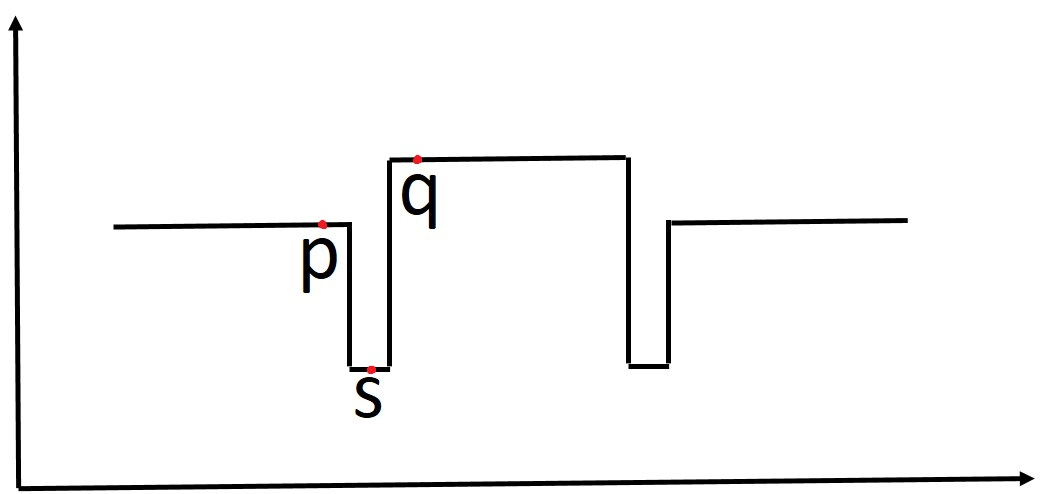
\includegraphics[width = 5.0cm]{results/Relation/relation.jpg}
\vspace{0.5mm}
\caption{ The relation between bilateral filtering and ours(change).}
\label{Fig:relation}
\end{figure}

\begin{figure}
\centering

\includegraphics[width = 7.0cm]{results/smileface.jpg}
\vspace{0.5mm}
\caption{ Explain the shortest path.}
\label{Fig:shortestpath}
\end{figure}

Our intrinsic filtering builds connections between $p$ and $q$, which providing more reliable information about the structure of the desired output.
This relation can be depicted in Figure \ref{Fig:relation}.
Our method inherits the advantage of these filtering algorithms~\cite{tomasi1998bilateral, grazzini2009edge, Chang2015propagated} while compensating their deficiencies,
and becomes more adaptive to the context of input signals.


\subsection{Filtering mesh geometry}

Given a noisy triangle mesh, our goal is to filter the noise while keeping the mesh structure.
In order to achieve this purpose, we adapt a two-stage process which be widely used in mesh filtering.
Firstly, noisy face normals are filtered iteratively by our intrinsic filtering model. %by equation~\ref{Eq:IntrinsicMeshFiltering}.
Secondly, according to the filtered face normals, vertex positions are updated iteratively though gradient descent.

{\bfseries Filtering face normals.}
When we consider normals as a surface signal defined over the original triangle mesh, it is easy to put the intrinsic filtering algorithm to mesh denoising.
For a triangle face $f_{i}$, its outward normal $\mathbf{n_{i}}$ can be calculated by outer product easily.
Then we consider $\mathbf{n_{i}}$ as a signal associated with the face centroid $c_{i}$.
In order to filter the face normals $\mathbf{n_{i}}$, we need find a path $L$ to connect $\mathbf{n_{i}}$ and its neighbor $\mathbf{n_{j}}$.
Finally, a filtered face normal $\bar{\mathbf{n_{i}}}$ is computed through our intrinsic mesh filtering model:
 \begin{equation}
 \label{Eq:IntrinsicMeshFiltering}
 \bar{\mathbf{n_{i}}} = \frac{1}{W_{i}}\sum_{\mathclap{f_{j}\in\mathcal{N}_{i}}}A_{j}g(d^{s}(\mathbf{n_{i}}, \mathbf{n_{j}}); \sigma_{s})g(d^{r}(\mathbf{n_{i}}, \mathbf{n_{j}}); \sigma_{r})\mathbf{n_{j}}\, .
 \end{equation}
  here,
 \begin{equation}
 \label{eq:IntrinsicMeshDistance}
 \left \{
 \begin{array}{ll}
        d^{s}(\mathbf{n_{i}}, \mathbf{n_{j}}) = (\sum_{x, x+1\in{L}}||\mathbf{n_{x+1}}-\mathbf{n_{x}}||^{n}\,\,)^{1/n} \vspace{1.5mm} \\
        d^{r}(\mathbf{n_{i}}, \mathbf{n_{j}}) = (\sum_{x\in{L}}||\mathbf{n_{x}}-\mathbf{n_{i}}||^{m}\,\,)^{1/m} \\
 \end{array}
 \right. ,
 \end{equation}
where $W_{i}$ is the normalization factor,
calculated by
$||\sum\limits_{\mathclap{f_{j}\in\mathcal{N}_{i}}}A_{j}g(d^{a}(\mathbf{n_{i}}, \mathbf{n_{j}}); \sigma_{s})g(d^{r}(\mathbf{n_{i}}, \mathbf{n_{j}}); \sigma_{r})||$
which ensures that $\bar{\mathbf{n_{i}}}$ is a unit normal;
$A_j$ is the area of face $f_j$;
$\mathcal{N}_{i}$ is the neighborhood of face $f_{i}$.
In our paper, we use the geometrical neighborhood, defined at the paper~\cite{Zhang2015Filter}.

Note that equation \ref{Eq:IntrinsicMeshFiltering} can be derived from equation \ref{Eq:GeneralForm}.
$A_j$ is the accumulation of infinitesimal area because the domain of integration is triangle face.
Furthermore, we give up the step length which measures the distance between adjacent centroid of triangle faces. % to facilitate the calculation in equation \ref{eq:IntrinsicMeshDistance}.
We simply make this term be one for facilitating the calculation.

Although the geodesic algorithm gives the shortest distance $d^s$ and $d^r$, it is computationally expensive.
Considering the shortcomings, we introduce a simple, fast and effective pattern for choosing filtering paths which is shown in next section.
We find that this operation is about an order of magnitude faster than applying shortest path in obtaining similar results.
Furthermore, the filter results that applying the particular paths often are more powerful on dealing with details, like edges and corners.
These results are shown in the figure \ref{Fig:shortestpath}.

\begin{figure}%[htb]
\centering
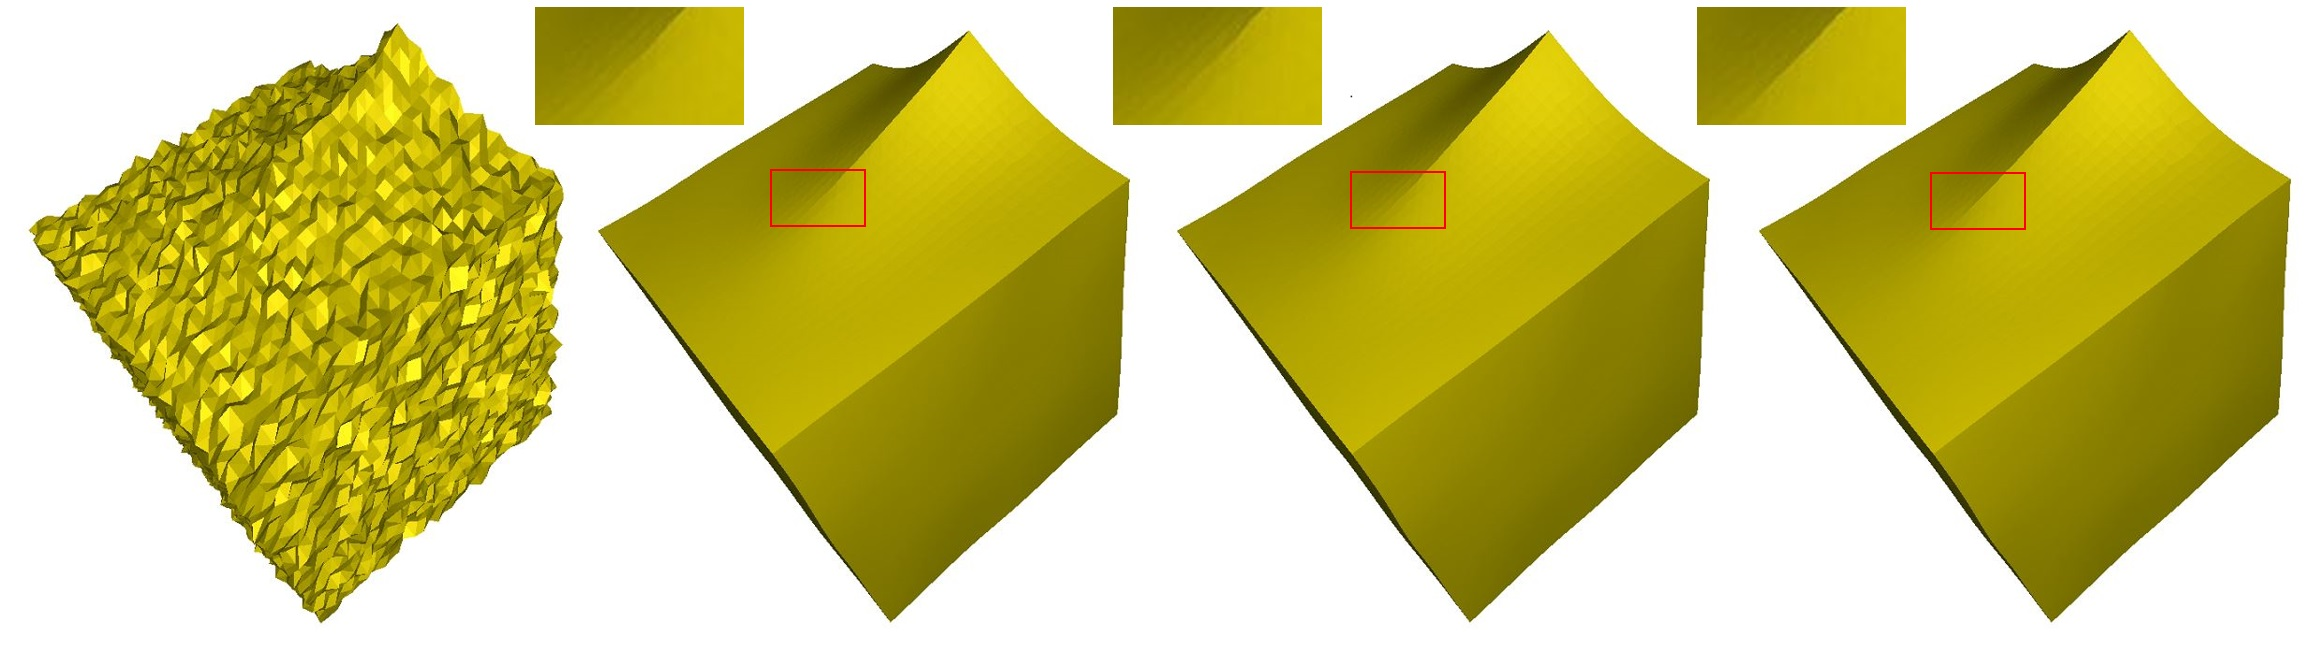
\includegraphics[width = 7.5cm]{results/Norm/norm.jpg}
\vspace{0.5mm}
\caption{ From the left to right: Noised mesh ( Gaussian noise with 0.3$\sigma_E$ ), the results of $m = n = 2$ with step length,
$m = n = 2$ without step length, $m = n = 1$ without step length.
Because of the sparseness of mesh feature, $L_1$ norm receives the best results in preserving the mesh structure.}
\label{Fig:norm}
\end{figure}

For triangle mesh, we conduct the experiment in the presence of $m$ and $n$ taking different values.
We mainly implement three group experiments. Figure~\ref{Fig:norm} show the denoised results of different conditions.
We find that $m=1$ and $n=1$ can obtain the best results because of the sparseness of mesh feature.
From the figure~\ref{Fig:norm}, the $L_1$ norm is more sensitive to details, so has a better expression.

 {\bfseries Updating vertices.} After all face normals is filtered, the vertex positions need to be updated to cater to these new normals.
 We adopt the iterative scheme in the paper~\cite{sun2007fast} to update the vertex positions.
 Namely, for a face $f_{i}$, we calculate its updated vertex positions via the following iteration form
 \begin{equation}
 \label{vertexupdate}
 \bar{v_{i}}^{(t+1)} = \bar{v_{i}}^{(t)} + \frac{1}{|{\mathcal{F}_{i}}|}\sum_{j\in\mathcal{F}_{i}}\mathbf{\bar{n}_{j}}[\mathbf{\bar{n}_{j}}\cdot(\bar{c_{j}}^{(t)}-\bar{v_{j}}^{(t)})]\, ,
 \end{equation}
 where $\bar{v_{j}}^{(t)}$ is the value of $\bar{v_{i}}$ in the $t-th$ iteration,
 $\mathcal{F}_{i}$ is the index set of the incident faces for $\bar{v_{i}}$,
 $|\cdot|$ denotes the cardinality of a set,
 and $\bar{c_{j}}^{(t)} = \sum_{i=1}^{3}\bar{v_{j_{i}}}^{(t)}/3$ is the centroid of the triangle $f_{j}$.
 This scheme is actually based on the orthogonality between the normal and the three edges of each face on the mesh.
 Then adopts a gradient descend process for solving that orthogonality equation in the conditions of  $L_2$ error.

 In our experiments, 10 to 20 iterations are sufficient for achieving satisfactory results and approximately up to above conditions.
 Our filtered process is summarized in Algorithm~\ref{alg:1}.
 In the next section, we introduce a simple but effective method for selecting a particular pattern for our propagated mesh filtering.



\begin{algorithm}\caption{Propagation mesh filtering framework}
\label{alg:1}
\begin{algorithmic}
\STATE {\textbf{Input:} Initial mesh $M_{in}$, number of iterations $k_{iter}$.}
\STATE{\textbf{Output:} Filtered mesh $M_{out}$.}
\STATE{1: $M^{(0)} = M_{in}$}
\STATE{2: \textbf{for} $s = 1$ to $k_{iter}$ \textbf{do}}
\STATE{3: ~~~Compute face normals {$n_i$} of mesh $M^{(s-1)}$;}
\STATE{4: ~~~Get paths from {$\mathcal{N}_i$} to {$n_i$} according to section \ref{Sec:path};}
\STATE{5: ~~~Compute filtered normals {$\mathbf{\bar{n_i}}$} according to~\ref{Eq:IntrinsicMeshFiltering};}
\STATE{6: ~~~Compute updated mesh $M^{(s)}$ according to {$\mathbf{\bar{n_i}}$};}
\STATE{7: \textbf{end for}}
\STATE{8: $M_{out} = M^{k_{iter}}$.}
\end{algorithmic}
\end{algorithm}



 \section{Path chosen for mesh filtering}
 \label{Sec:path}

\begin{figure}[htb]
\centering
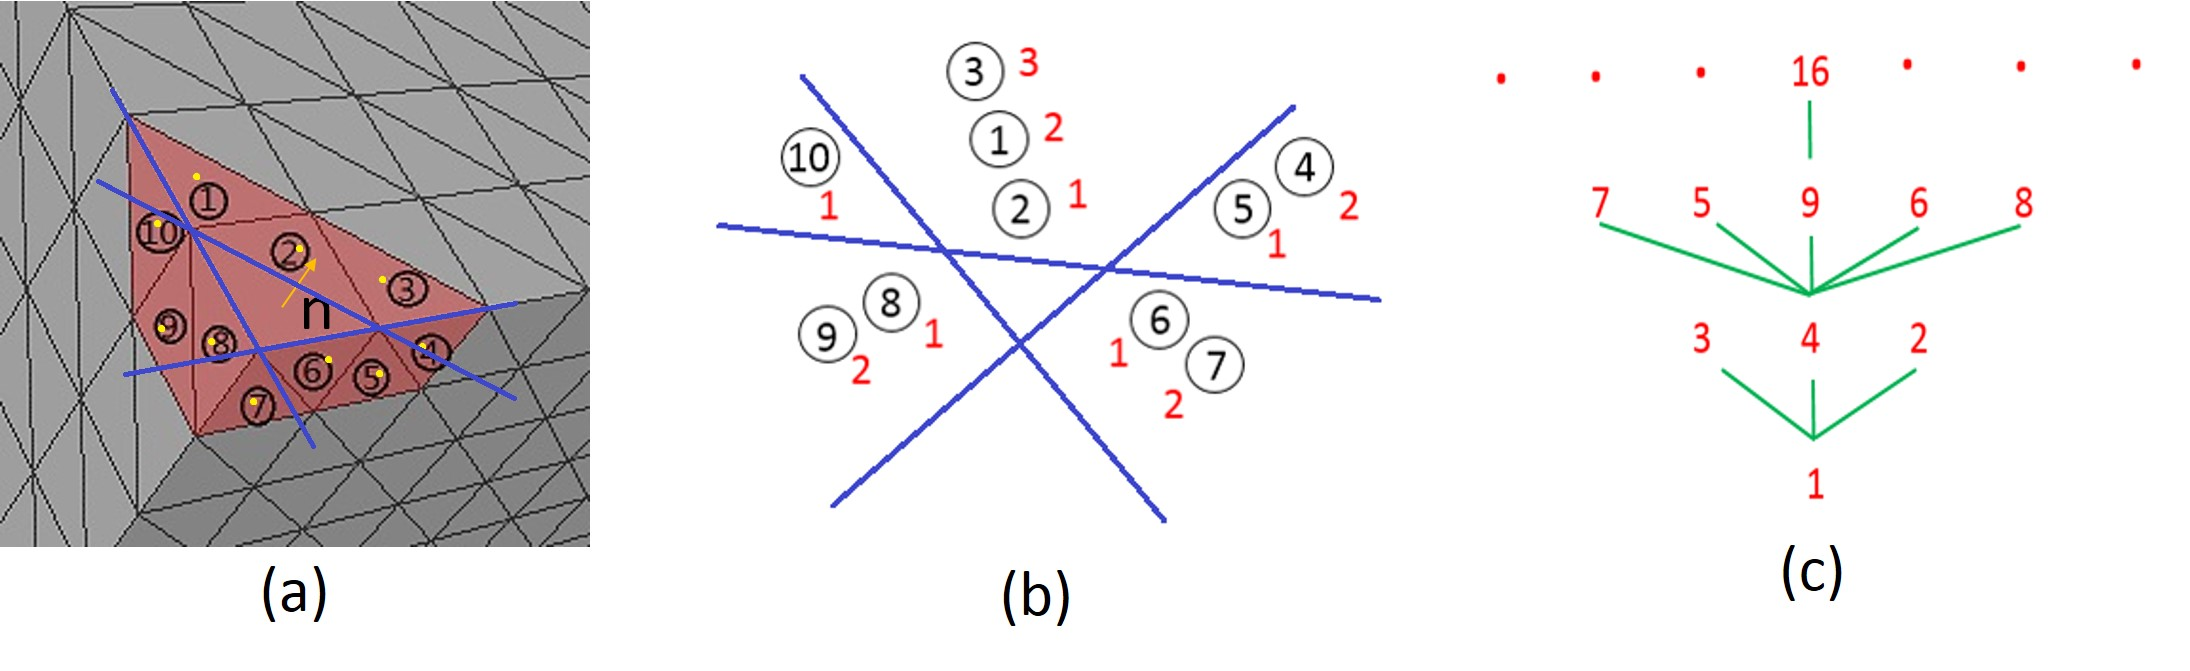
\includegraphics[width = 7.5cm]{results/Path/path1.jpg}
\vspace{-3mm}
\caption{ The process of generation path. (a) the 10 neighbors of current face with its normal $\mathbf{n}$. (b) The schematic diagram after projection, dividing and sorting. (c) the pattern.
The numbers with circle are the neighbor of current triangle face, the yellow points are the projection points of neighbor face centroid, the blue lines are used to decide the face label, the red numbers are their serial number after sorting, the green lines are connected path.}
\label{Fig:path}
\end{figure}

 In image, many particular patterns can be chosen because of the regular coordination system.
 These patterns are simple and easy to be thought about.
 But in triangle mesh, it is very difficult to obtain a good pattern which can preserve the mesh feature.
 The easiest way to be thought of is applying the shortest path algorithm on the triangle mesh.
 However, figure \ref{Fig:shortestpath} shows this method is time consuming.
 We solve this problem in this paper within the context of mesh denoising.

 Our method is based on the following theory: the areal coordinates of triangle segments the plane into seven regions.
 Areal coordinates are extremely useful in engineering applications involving triangular subdomains.
 These make analytic integrals often easier to evaluate, and Gaussian quadrature tables are often presented in terms of area coordinates.
 In the context of a triangle, the areal coordinates of a point $P$ are the ratios of the areas of $PBC$, $PCA$ and $PAB$ to the area of the reference triangle $ABC$.
 %shown in the figure~\ref{Fig:path}(a).
 Because the ratios are a plus or a minus, it divide the plane where the triangle is to seven parts.
 That gives us an enlightenment to obtain a particular pattern for solving the problem of paths.

{\bfseries Path generation.}
For each triangle $f_i$, we project its neighborhood $\mathcal{N}_i$ onto a tangent plane basing its normal $\mathbf{\bar{n_i}}$.
In detail, we only project their centroid onto that plane.
Then basing the three points of $f_i$, we use areal coordinations to divide these centroid to seven regions.
Note that, if the projection point falls into the face $f_i$, we throw it away from $\mathcal{N}_i$.
In this way, we give each neighbor a label that belong to a specified region.
Afterwards, we sort these neighbors belong to the same region according to their face centroid distance to $c_i$ in original noisy mesh.
Finally, we provide a particular pattern to assign the path for matching the ordered neighbors.
This pattern is defined square-pattern, which is used for generating paths.
The entire process is depicted in the figure~\ref{Fig:path}.

{\bfseries Advantages.} 
 The above process has the power to protect local mesh feature like edge and corner.
 To a certain extend, the six regions surrounding $f_i$ depict the local structure of a mesh.
 Projecting along the normal of $f_i$ makes the faces having similar normal flock together.
 Furthermore, the division further restricts the normal difference according to areal coordinates.
 The combination of these two aspects insures that one of six regions has the similarity to $f_i$.
 The part including faces $\textcircled{1}$, $\textcircled{2}$ and $\textcircled{3}$ has the similar normal to $f_i$ in the figure \ref{Fig:path}(b).
 These normals play a important role in applying our intrinsic filtering algorithm.

 Figure \ref{Fig:path}(c) shows the square-pattern for generating path.
 We use $n^2$($ n = 1, 2,...$) as connection points, the sequence numbers between $(m-1)^2$ and $m^2$ including $m^2$ directly connect the number $(m-1)^2$.
 In this way, paths are generated.
 For example, the path between number $8$ and $f_i$ is $8-4-1-f_i$, number $16$ and $f_i$ is $16-9-4-1-f_i$ and so on.

 In the next section, we will introduce the experimental results basing our method.
\section{Implementation and results}
\subsection{Parameters chosen}

\begin{figure}
\centering
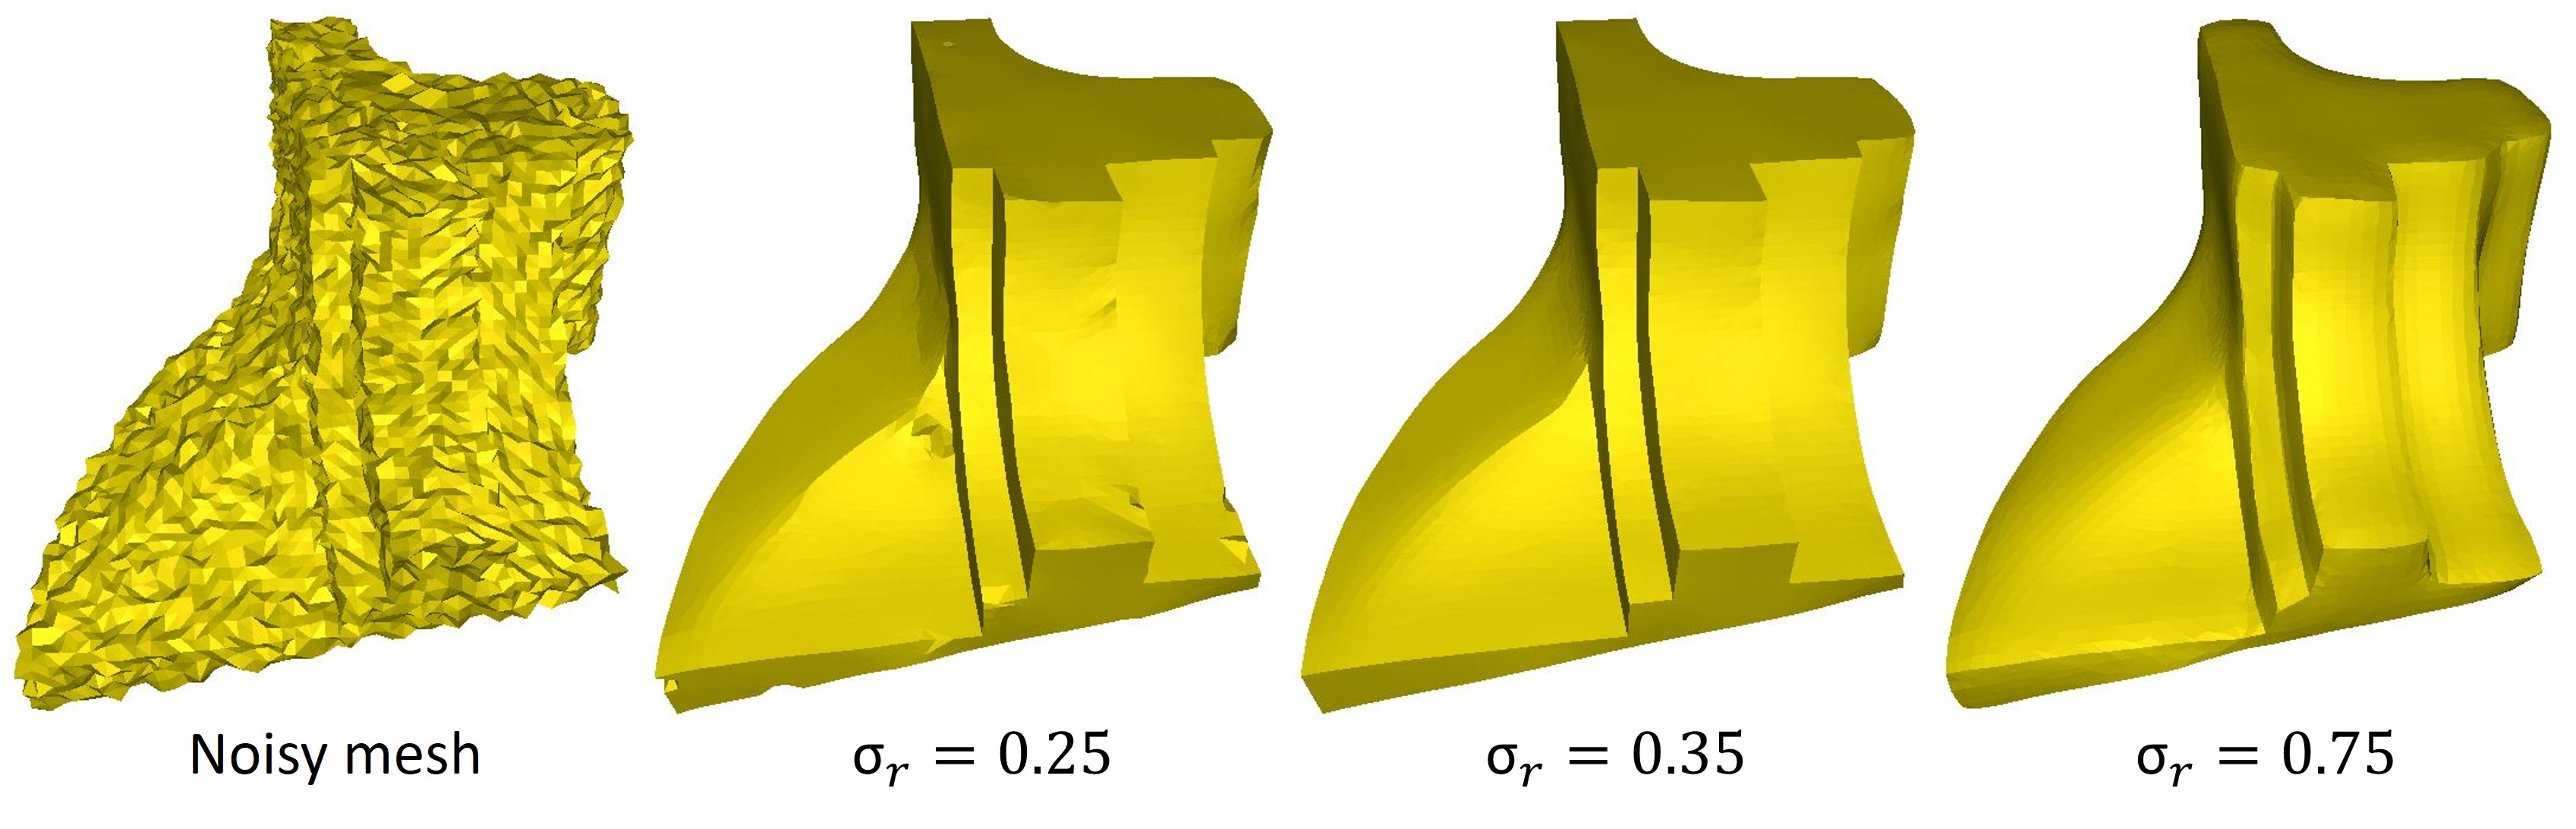
\includegraphics[width = 7.5cm]{results/SigmaR/sigma_r.jpg}
\vspace{-0.5mm}
\caption{ Denoising results using different values of $\sigma_r$ with other parameters fixed ($k_{iter} = 30$, $v_{iter} = 2$, $r = 4$).}
\label{Fig:sigma}
\end{figure}

\begin{figure}
\centering
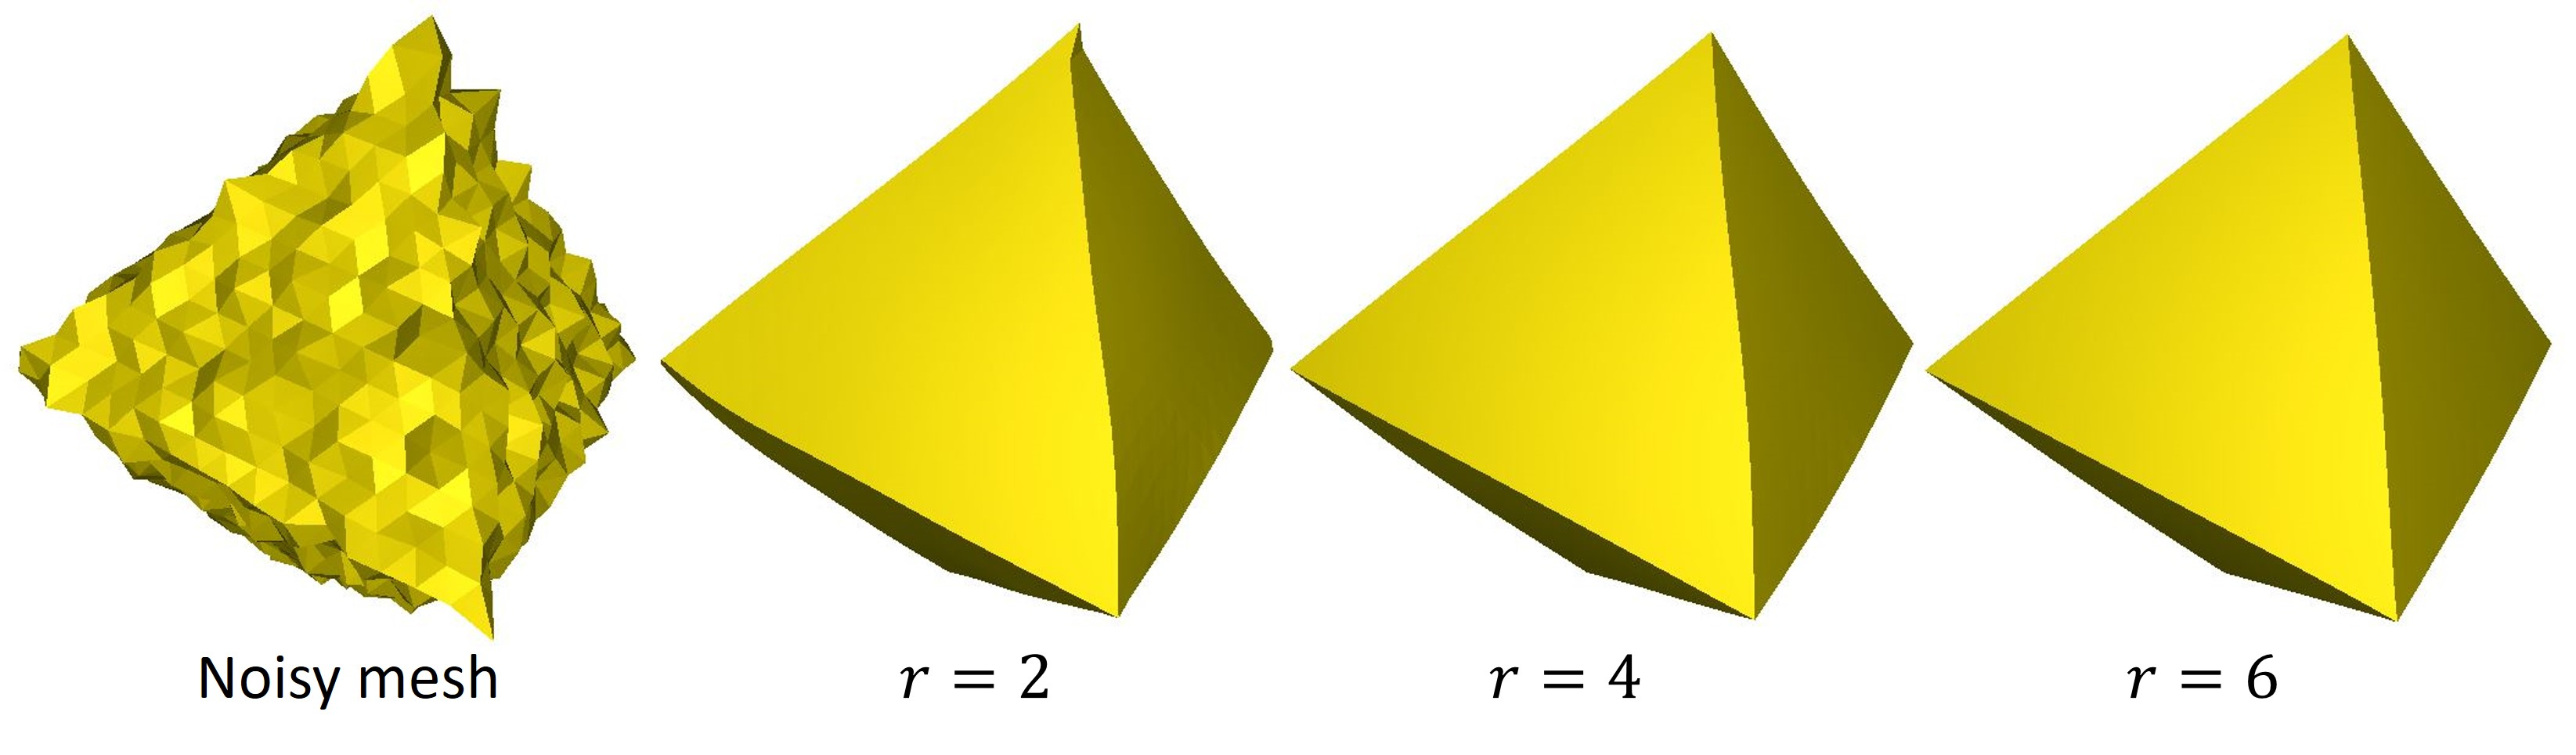
\includegraphics[width = 7.5cm]{results/Radius/radius.jpg}
\vspace{-1mm}
\caption{ Denoising results using different values of $r$ with other parameters fixed ($k_{iter} = 75$, $v_{iter} = 2$, $\sigma_r = 0.28$).
The corresponding error $E_v$ is 0.0049, 0.0038 and 0.0030, $E_n$ is 2.35, 1.67 and 1.00 respectively.\jj{change line graph?}  }
\label{Fig:radius}
\end{figure}

%\begin{figure*}
%\centering
%
%\subfigure
%{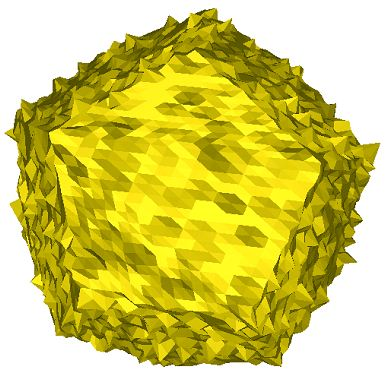
\includegraphics[width = 1.8cm]{results/TwelveIm0.5/snapshot00.jpg}}
%\subfigure
%{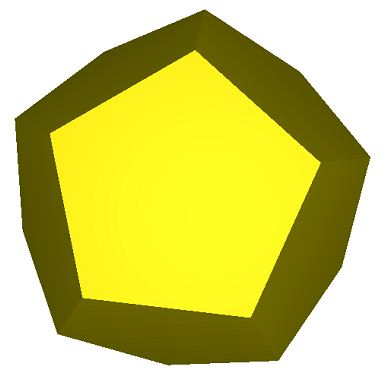
\includegraphics[width = 1.8cm]{results/TwelveIm0.5/snapshot01.jpg}}
%\subfigure
%{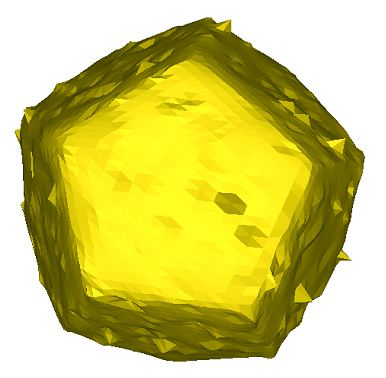
\includegraphics[width = 1.8cm]{results/TwelveIm0.5/snapshot02.jpg}}
%\subfigure
%{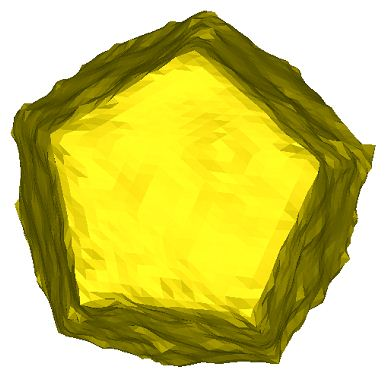
\includegraphics[width = 1.8cm]{results/TwelveIm0.5/snapshot03.jpg}}
%\subfigure
%{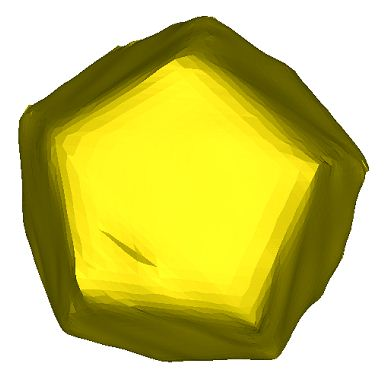
\includegraphics[width = 1.8cm]{results/TwelveIm0.5/snapshot04.jpg}}
%\subfigure
%{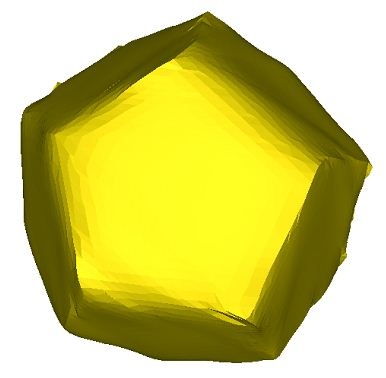
\includegraphics[width = 1.8cm]{results/TwelveIm0.5/snapshot05.jpg}}
%\subfigure
%{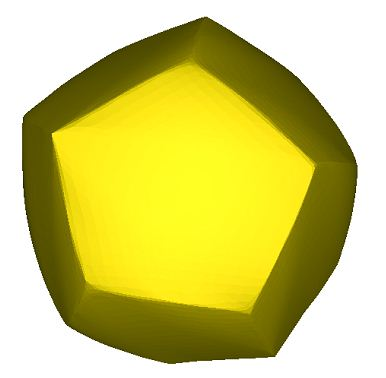
\includegraphics[width = 1.8cm]{results/TwelveIm0.5/snapshot06.jpg}}
%\subfigure
%{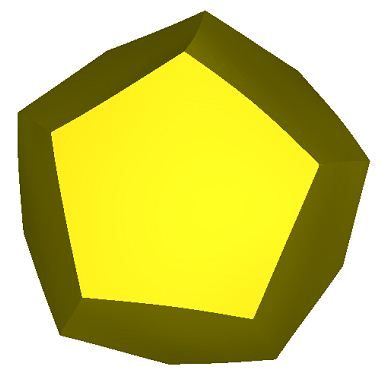
\includegraphics[width = 1.8cm]{results/TwelveIm0.5/snapshot07.jpg}}
%\subfigure
%{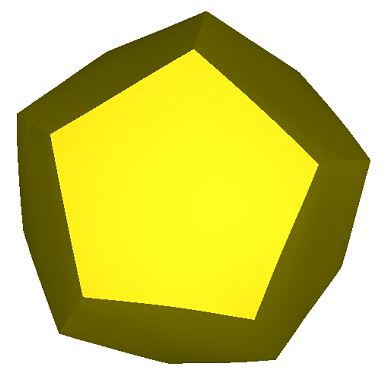
\includegraphics[width = 1.8cm]{results/TwelveIm0.5/snapshot08.jpg}}
%
%\caption{ Camparison of denoising algorithms on a mesh. The intensity $\sigma_E$ of the impulsive noise applied to this model is 0.5.
%The results are from left to right noisy mesh, original mesh
%, \cite{fleishman2003bilateral}, \cite{jones2003non}, \cite{sun2007fast}, \cite{zheng2011bilateral}(l), \cite{he2013mesh}, \cite{Zhang2015Filter} and ours respectively.}
%\label{Fig:Impulsive}
%\end{figure*}

Our method has four parameters: the number of normal filtering iterations $k_{iter}$,
the number of iterations $v_{iter}$ for vertex update,
choosing a radius parameter $r$ determined the geometrical neighborhood,
and the standard variance parameters $\sigma_s$ and $\sigma_r$, for the two difference between normals, respectively.
In our experiments, we find that $k_{iter}\leq75$ and $v_{iter}\leq5$ are enough for achieving satisfactory results.
For all results in this paper, we set the same value to $\sigma_s$ and $\sigma_r$ for employing the filtering unless stated otherwise.
As the $\sigma_s$ and $\sigma_r$ control the integral of two kinds of normal difference,
small value can retain details, for example weak edge, but some noise can not be removed;
big value can remove noise but weaken some features (Fig.\ref{Fig:sigma}).
So we need tune their values to achieve a good experimental result.
For most meshes, we choose their values between 0.1 and 0.8.
In addition, we choose $r\in[2d, 6d]$ where $d$ is the average distance between neighboring face centroid across the whole mesh.
For CAD model, the two error metrics introduced in next section will decrease with increase of $r$ seen in figure~\ref{Fig:radius},
so bigger $r$ obtains more satisfactory experimental results.
The reason is that some one of six regions provides more reliable normal estimation.


\subsection{Results and comparisons}

In the following, we compare our mesh denoising strategy with other methods basing the vertex filtering~\cite{fleishman2003bilateral}, normal filtering~\cite{jones2003non, sun2007fast, zheng2011bilateral, Zhang2015Filter} and $L_0$ minimization~\cite{he2013mesh} on synthetic and real noisy meshes.
\cite{zheng2011bilateral} proposes two denoising scheme: a local scheme and a global scheme.
Its local method uses bilateral normal filtering strategy and its global method solves the denoising problem by minimizing a energy function.
In this paper, we only compare with their local scheme.

We generate the synthetic meshes through adding noise to the vertices of a ground truth mesh along the vertex normals.
The intensity of the noise is defined by a relative standard deviation $\sigma_E = \sigma / E_{mean}$,
where $\sigma$ is the standard deviation of the Gaussian function and $E_{mean}$ is the average edge length of the ground truth mesh.
For a fair comparison, for each method we fine tune the parameters to produce the best results in their parameter space.
And furthermore, for synthetic meshes, we also evaluate two quantitative metrics about vertex-based and normal-based mesh-to-mesh error metric
respectively introduced in papers~\cite{belyaev2003comparison} and~\cite{nehorai2000performance} to analyze the difference between our results and others.
These two metrics measure mean deviations about vertex and face between denoised mesh and true mesh.

The vertex-based error metric is
\begin{equation}
\label{Eq:vertexerror}
E_v = \sqrt{\frac{1}{3 A(M^{'})}\sum_{P^{'} \in M^{'}} A(P^{'}) dist(P^{'}, M)^2}\, ,
\end{equation}
where $M$ and $M^{'}$ reference original noiseless mesh and denoised mesh respectively, $P^{'}$ is a vertex of $M^{'}$
and $dist(P^{'}, M)$ defines the distance between $P^{'}$ and a triangle of $M$ which is closest to $P^{'}$.

The normal-based error metric is used to reveal the average angle offset which is defined as follows
\begin{equation}
\label{Eq:normalerror}
E_n = \sum_{f^{'} \in M^{'}, f \in M} angle(\mathbf{n^{'}}, \mathbf{n}) / N\, ,
\end{equation}
where $f^{'}$ and $f$ are triangle faces of $M^{'}$ and $M$ respectively,
$\mathbf{n^{'}}$ and $\mathbf{n}$ reference the normal of $f^{'}$ and $f$,
$angle(\mathbf{n^{'}}, \mathbf{n})$ defines the angle between $\mathbf{n^{'}}$ and $\mathbf{n}$
and the last $N$ is the number of triangle faces of a mesh.

\begin{figure*}
\centering

\subfigure
{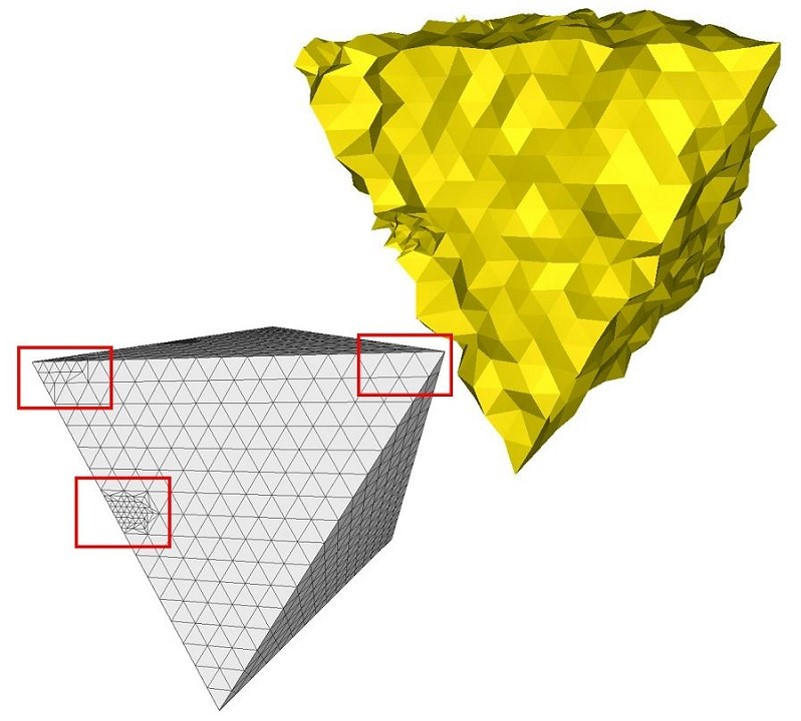
\includegraphics[width = 1.6cm]{results/Octahedron0.3/snapshot00C.jpg}}
\subfigure
{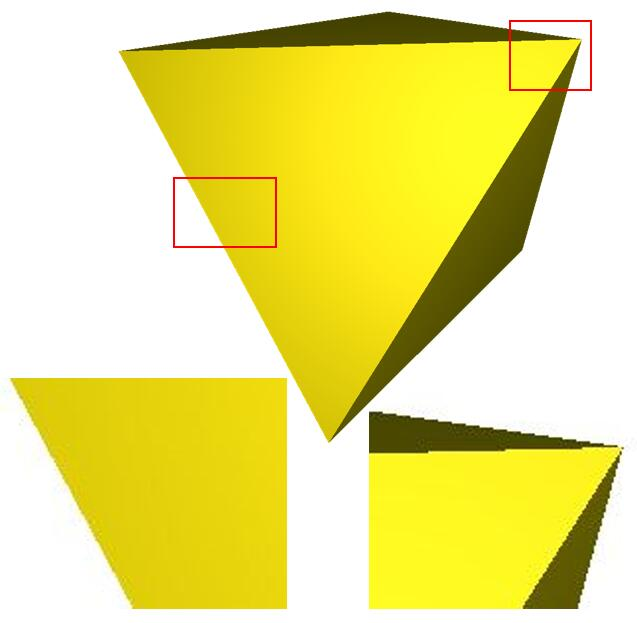
\includegraphics[width = 1.8cm]{results/Octahedron0.3/snapshot01C.jpg}}
\subfigure
{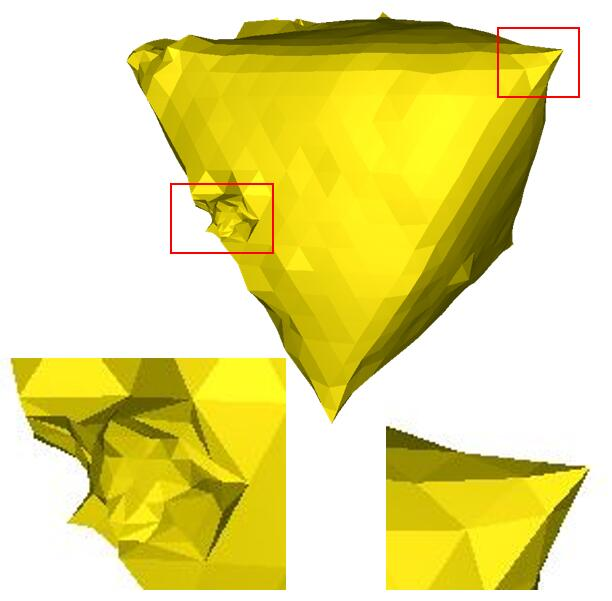
\includegraphics[width = 1.8cm]{results/Octahedron0.3/snapshot02C.jpg}}
\subfigure
{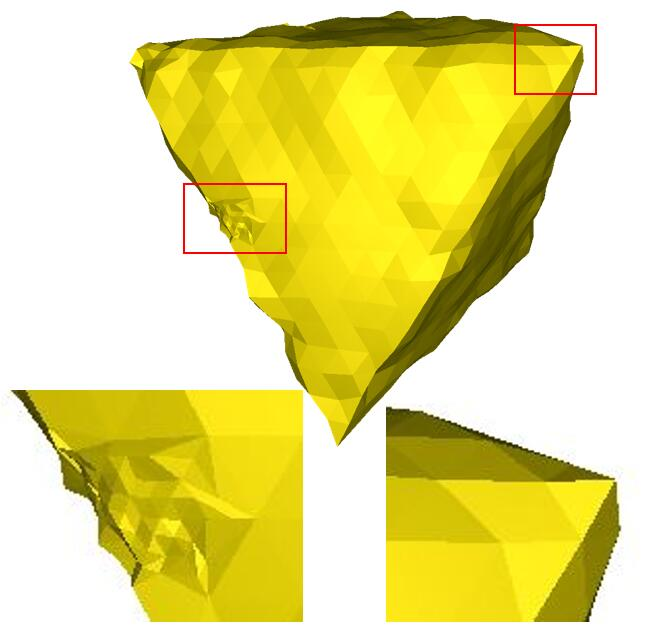
\includegraphics[width = 1.8cm]{results/Octahedron0.3/snapshot03C.jpg}}
\subfigure
{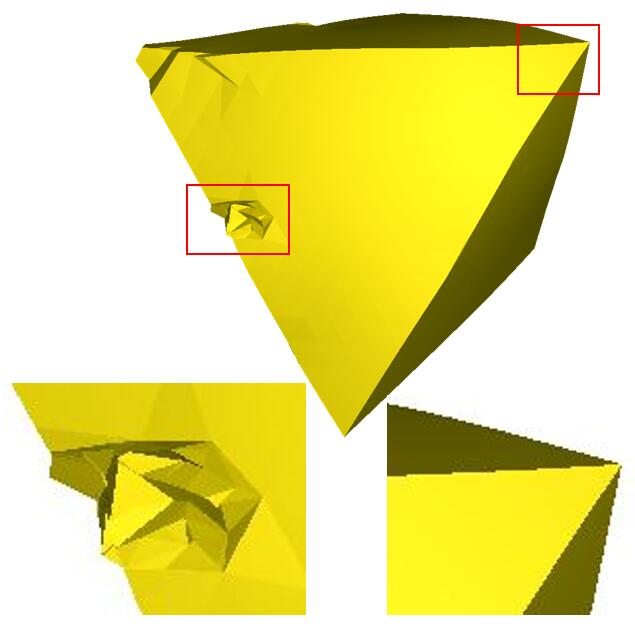
\includegraphics[width = 1.8cm]{results/Octahedron0.3/snapshot04C.jpg}}
\subfigure
{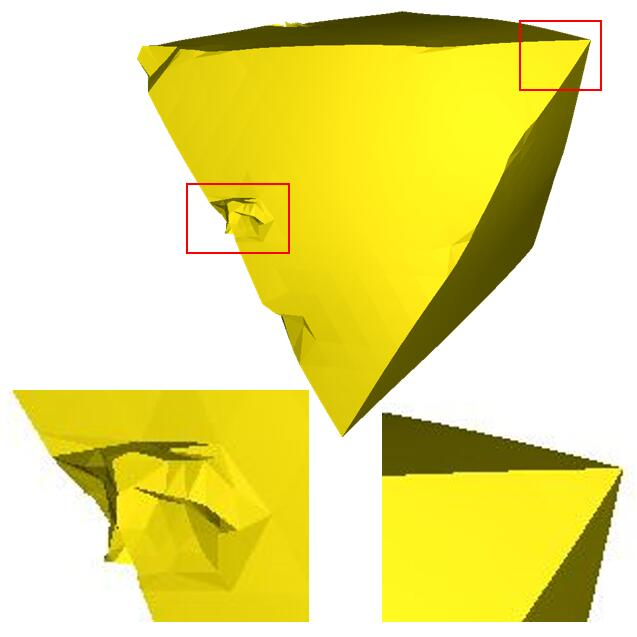
\includegraphics[width = 1.8cm]{results/Octahedron0.3/snapshot05C.jpg}}
\subfigure
{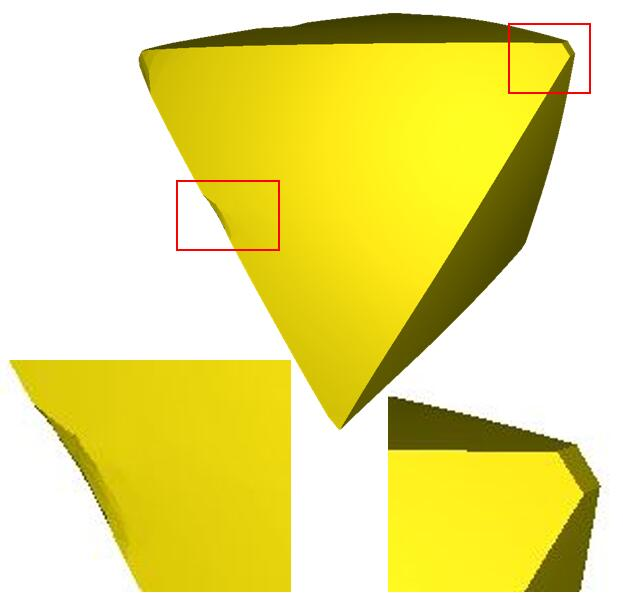
\includegraphics[width = 1.8cm]{results/Octahedron0.3/snapshot06C.jpg}}
\subfigure
{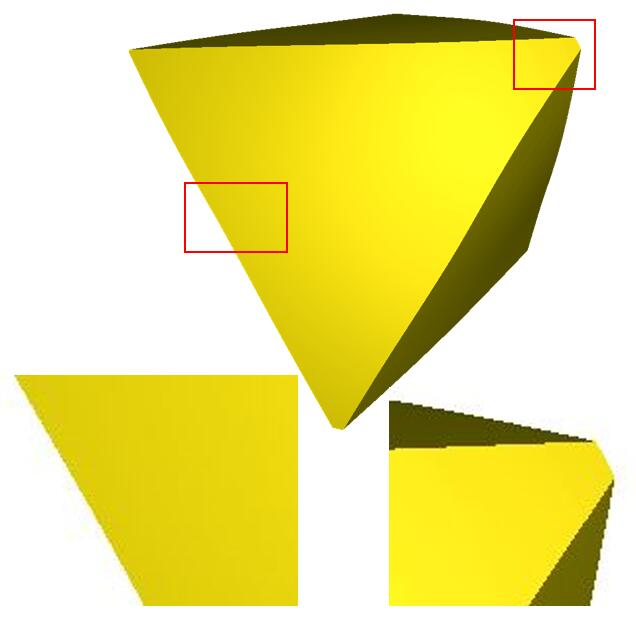
\includegraphics[width = 1.8cm]{results/Octahedron0.3/snapshot07C.jpg}}
\subfigure
{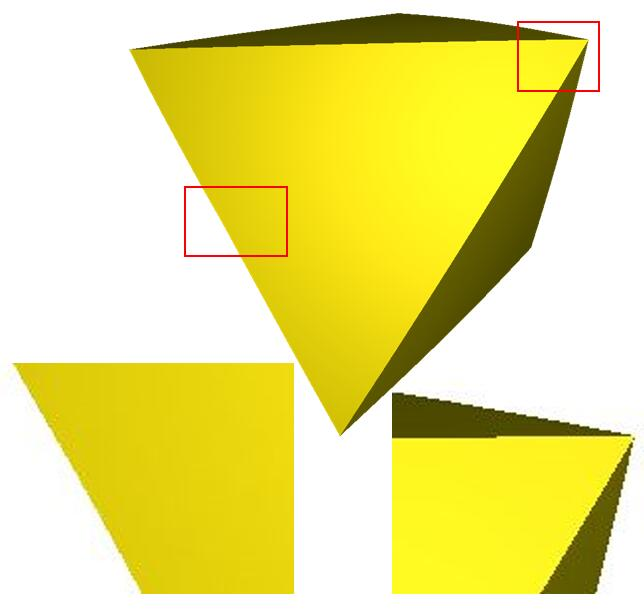
\includegraphics[width = 1.8cm]{results/Octahedron0.3/snapshot08C.jpg}}
\vspace{-1.2mm}
\caption{ Denoising a mesh with non-uniform sampling with the Gaussian noise intensity $\sigma_E = 0.3$.
The results are from left to right noisy mesh, original mesh
, \cite{fleishman2003bilateral}, \cite{jones2003non}, \cite{sun2007fast}, \cite{zheng2011bilateral}, \cite{he2013mesh}, \cite{Zhang2015Filter} and ours respectively.}
\label{Fig:octahedron}
\end{figure*}

\begin{figure*}
\centering

\subfigure
{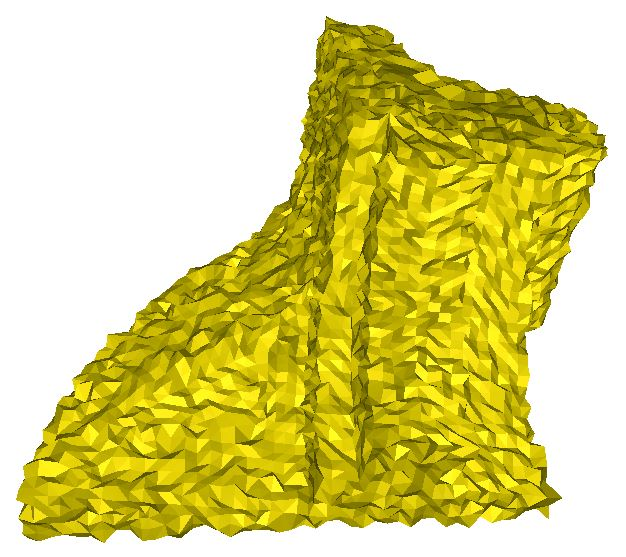
\includegraphics[width = 1.8cm]{results/Fandisk0.3/snapshot00.jpg}}
\subfigure
{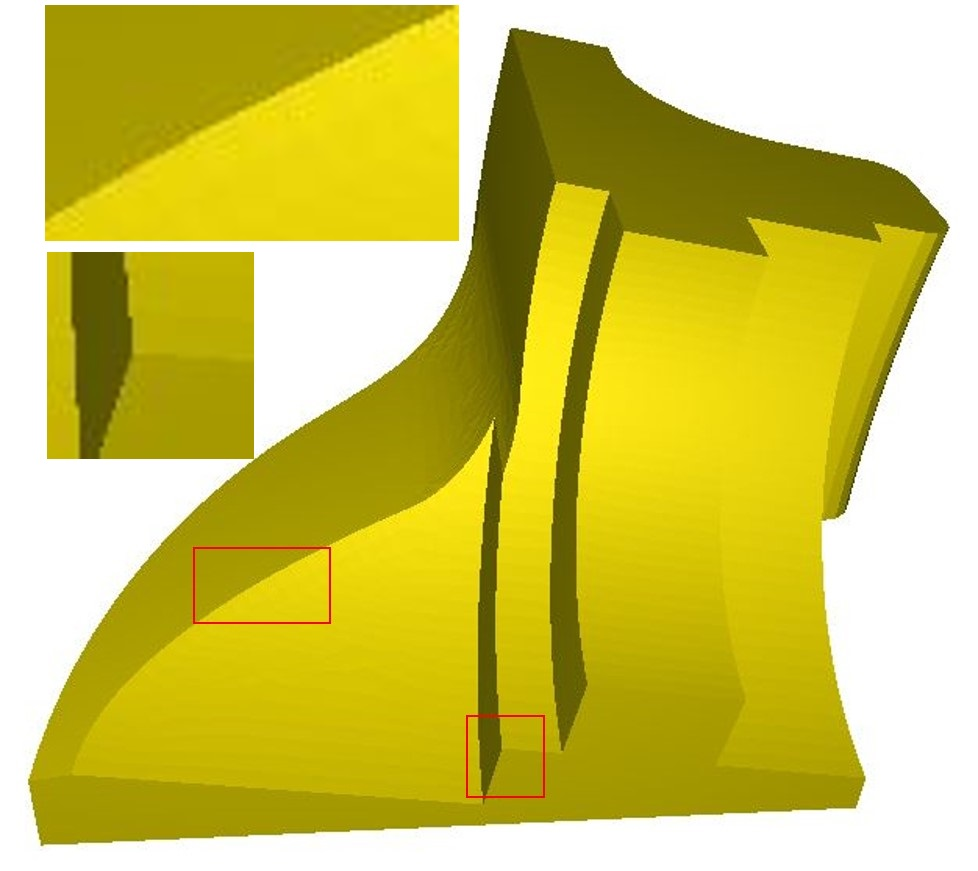
\includegraphics[width = 1.8cm]{results/Fandisk0.3/snapshot01.jpg}}
\subfigure
{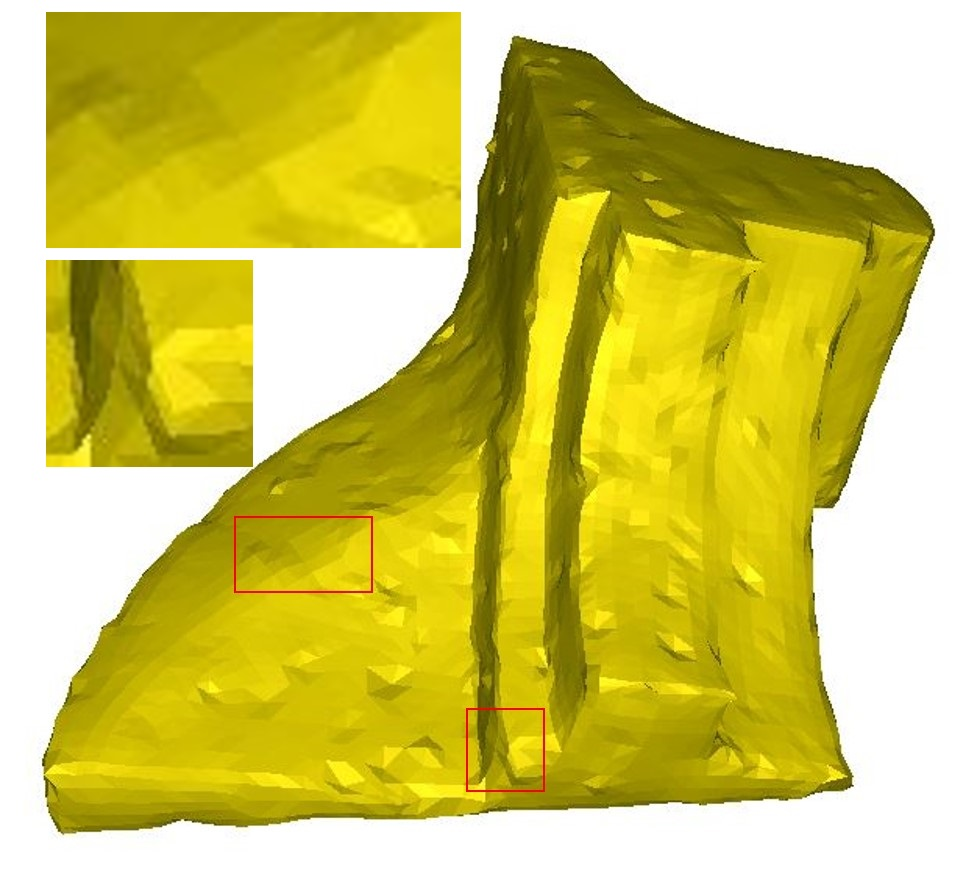
\includegraphics[width = 1.8cm]{results/Fandisk0.3/snapshot02.jpg}}
\subfigure
{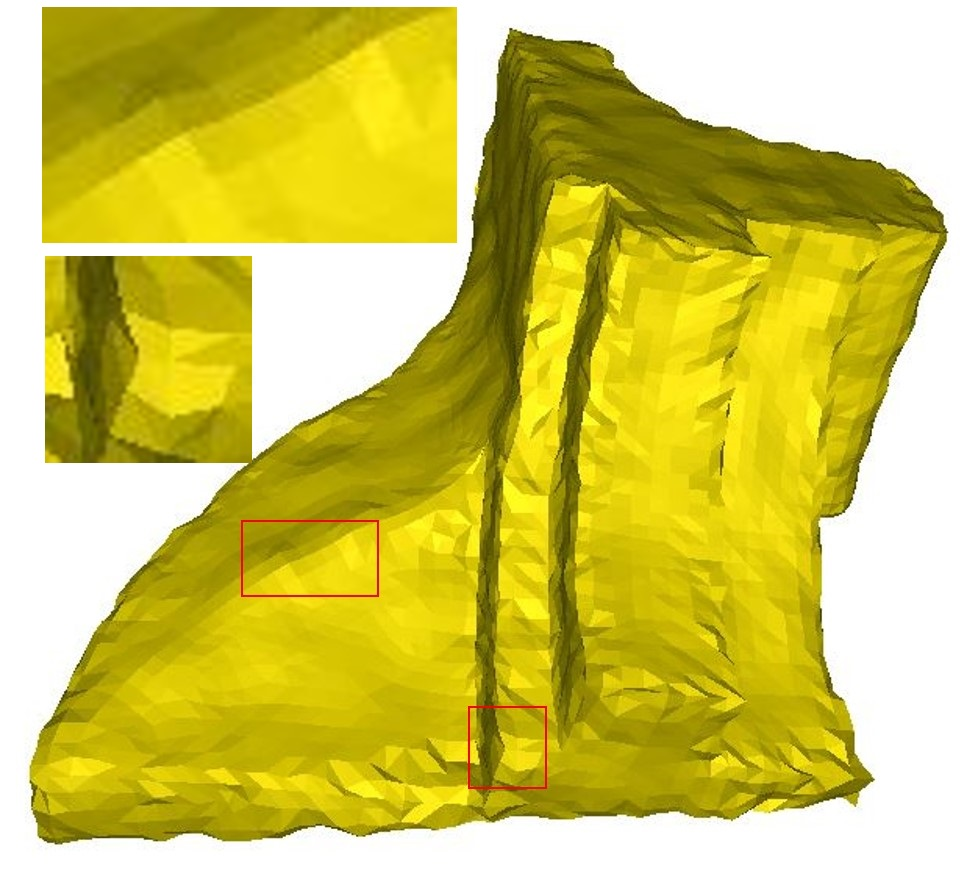
\includegraphics[width = 1.8cm]{results/Fandisk0.3/snapshot03.jpg}}
\subfigure
{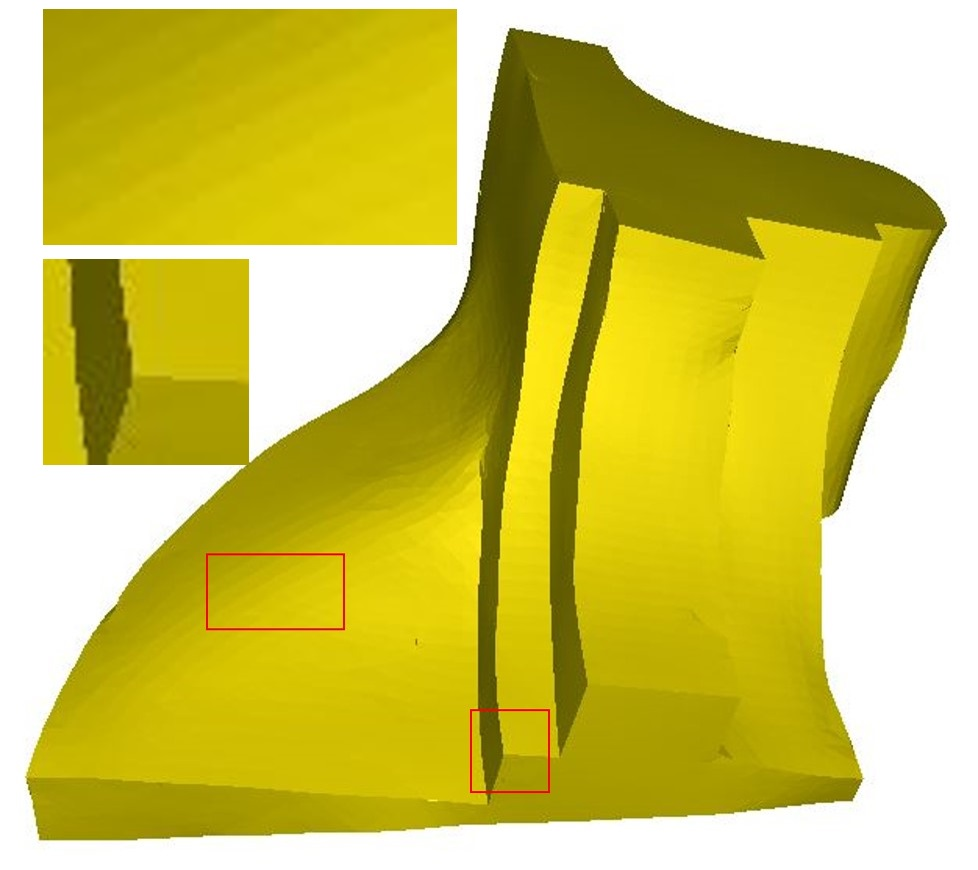
\includegraphics[width = 1.8cm]{results/Fandisk0.3/snapshot04.jpg}}
\subfigure
{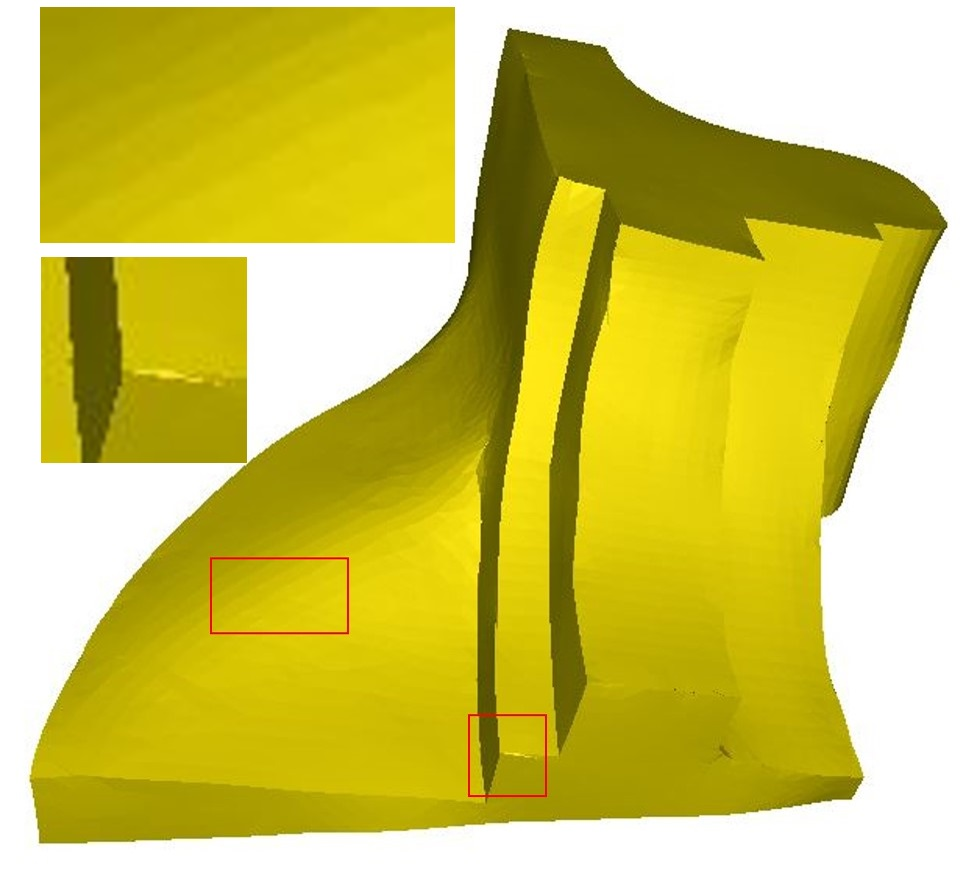
\includegraphics[width = 1.8cm]{results/Fandisk0.3/snapshot05.jpg}}
\subfigure
{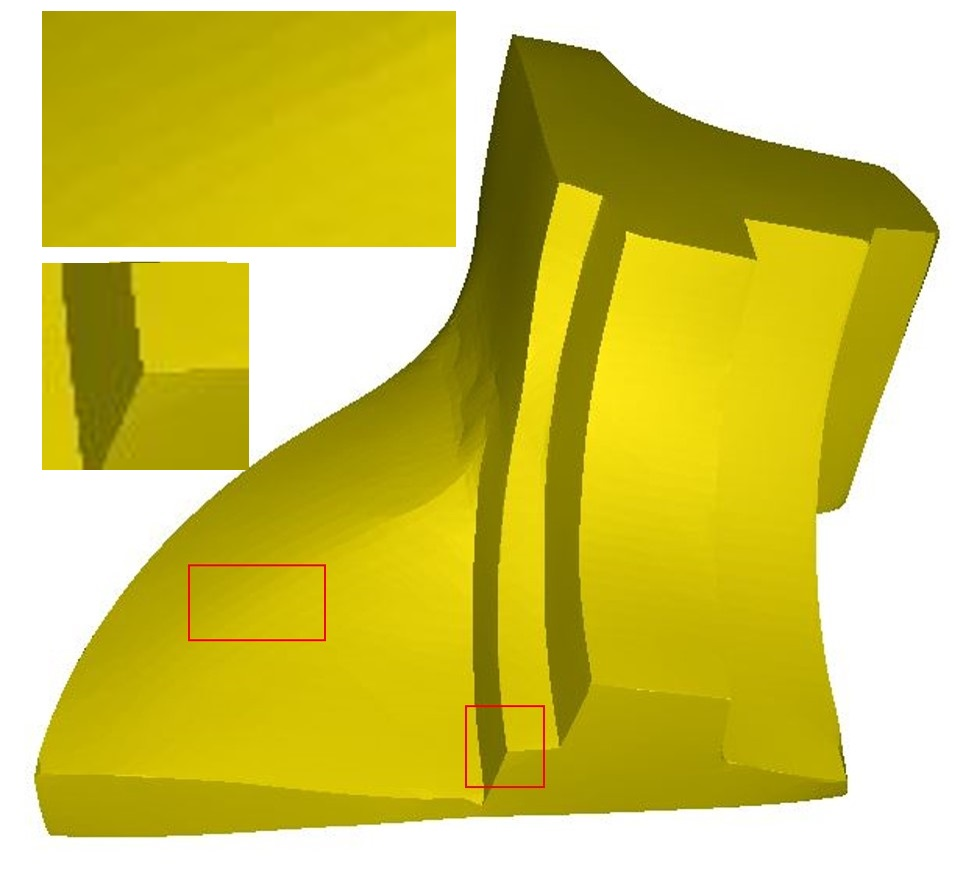
\includegraphics[width = 1.8cm]{results/Fandisk0.3/snapshot06.jpg}}
\subfigure
{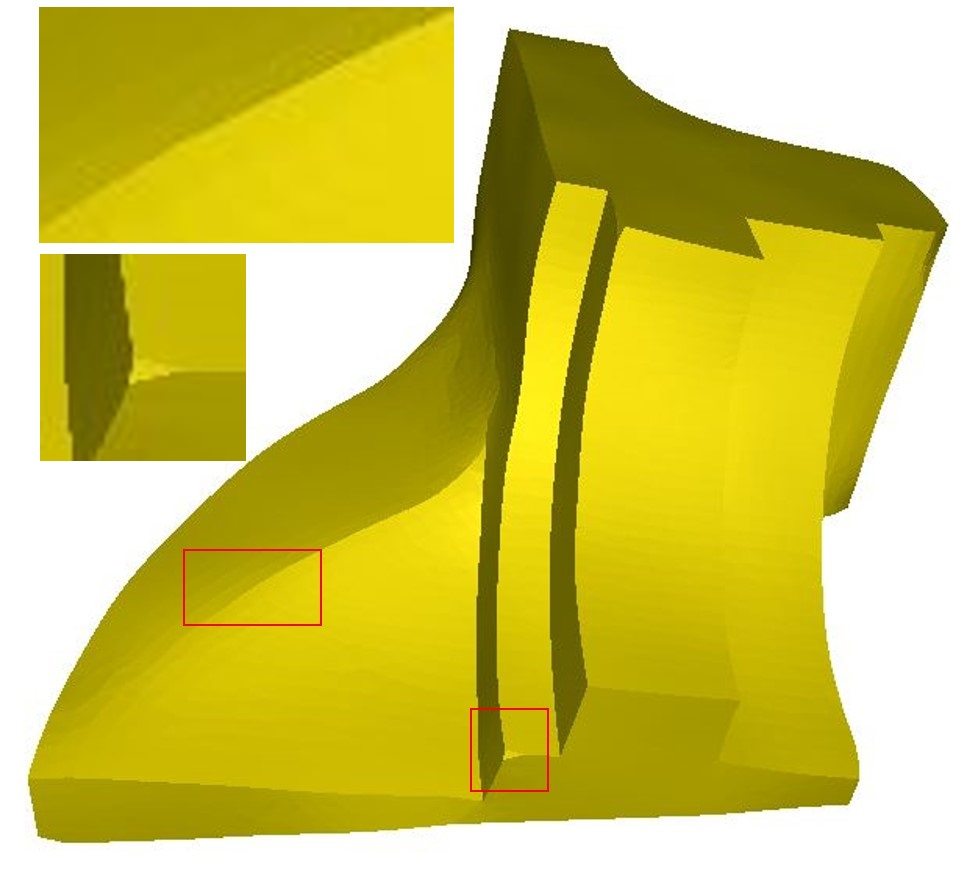
\includegraphics[width = 1.8cm]{results/Fandisk0.3/snapshot07.jpg}}
\subfigure
{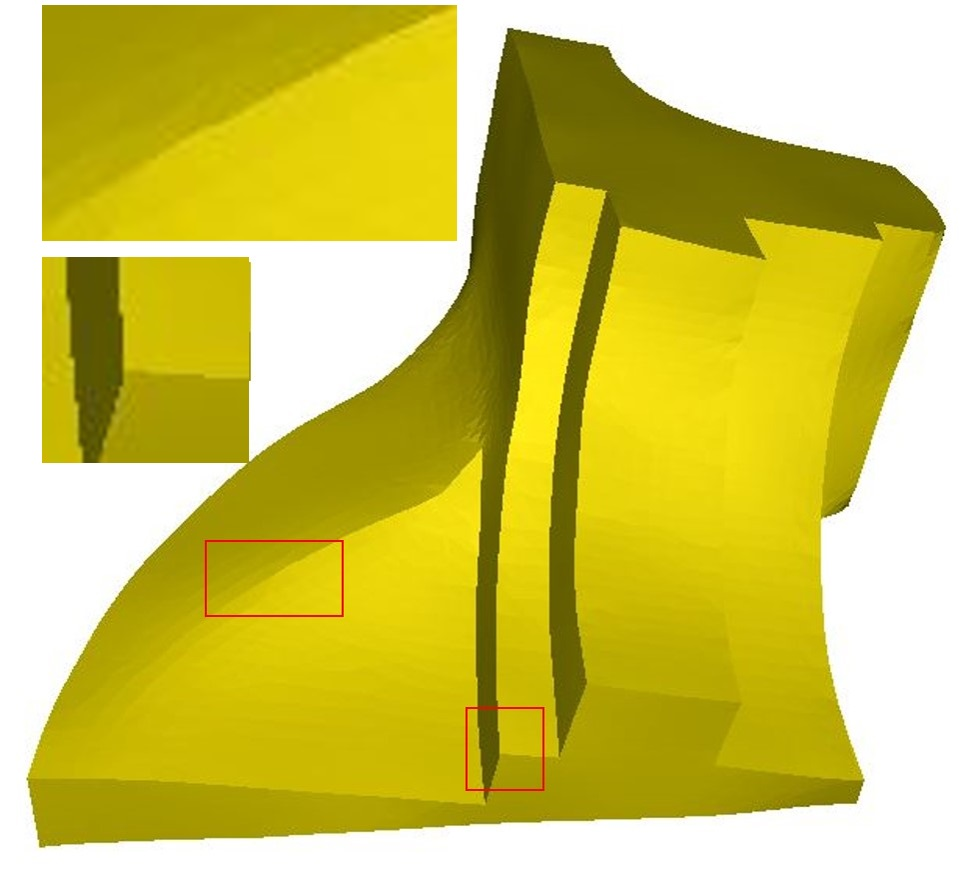
\includegraphics[width = 1.8cm]{results/Fandisk0.3/snapshot08.jpg}}
\\
\vspace{-1.2mm}

\subfigure
{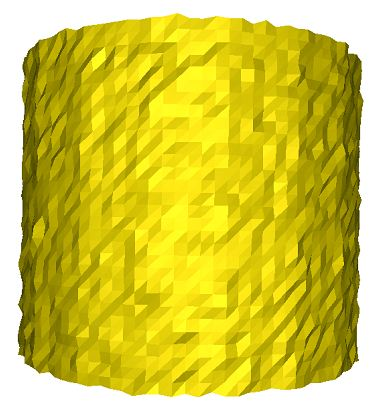
\includegraphics[width = 1.8cm]{results/Prism0.1/snapshot00.jpg}}
\subfigure
{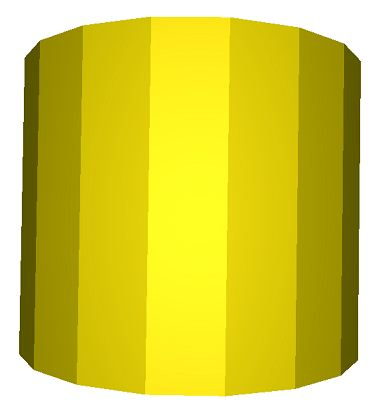
\includegraphics[width = 1.8cm]{results/Prism0.1/snapshot01.jpg}}
\subfigure
{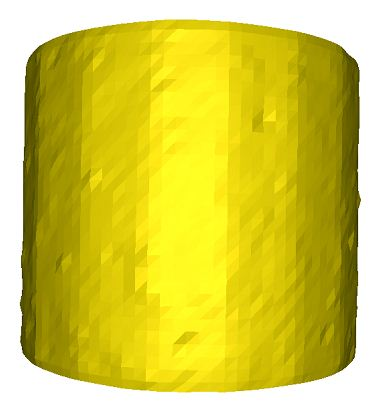
\includegraphics[width = 1.8cm]{results/Prism0.1/snapshot02.jpg}}
\subfigure
{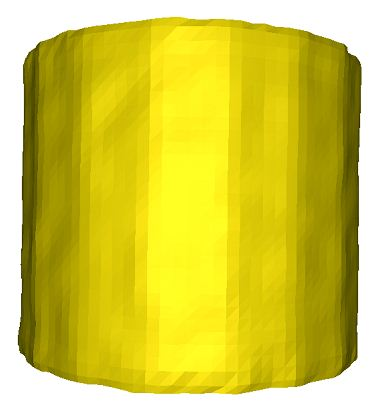
\includegraphics[width = 1.8cm]{results/Prism0.1/snapshot03.jpg}}
\subfigure
{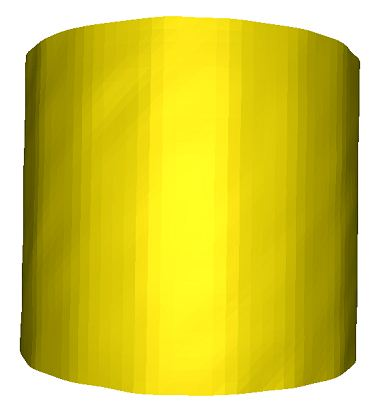
\includegraphics[width = 1.8cm]{results/Prism0.1/snapshot04.jpg}}
\subfigure
{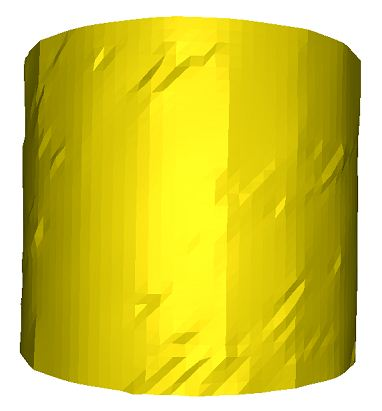
\includegraphics[width = 1.8cm]{results/Prism0.1/snapshot05.jpg}}
\subfigure
{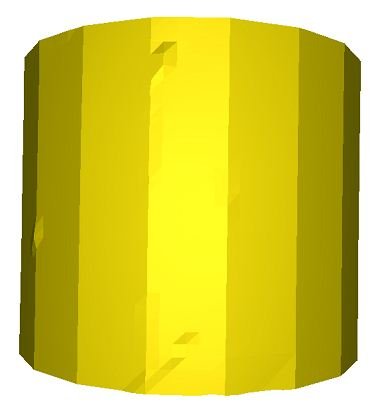
\includegraphics[width = 1.8cm]{results/Prism0.1/snapshot06.jpg}}
\subfigure
{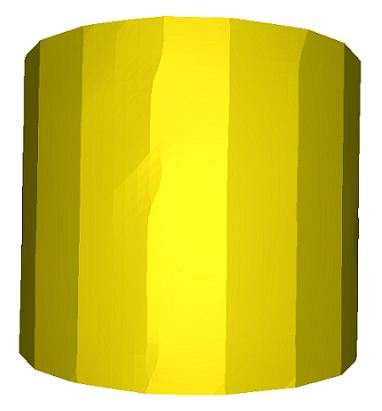
\includegraphics[width = 1.8cm]{results/Prism0.1/snapshot07.jpg}}
\subfigure
{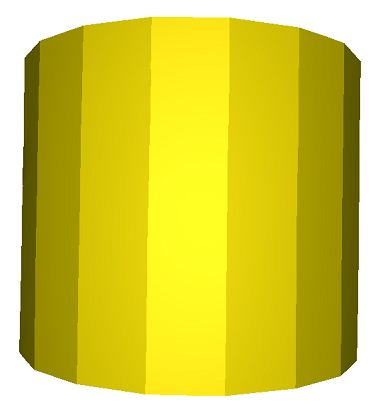
\includegraphics[width = 1.8cm]{results/Prism0.1/snapshot08.jpg}}
\\
\vspace{-1.2mm}

\subfigure
{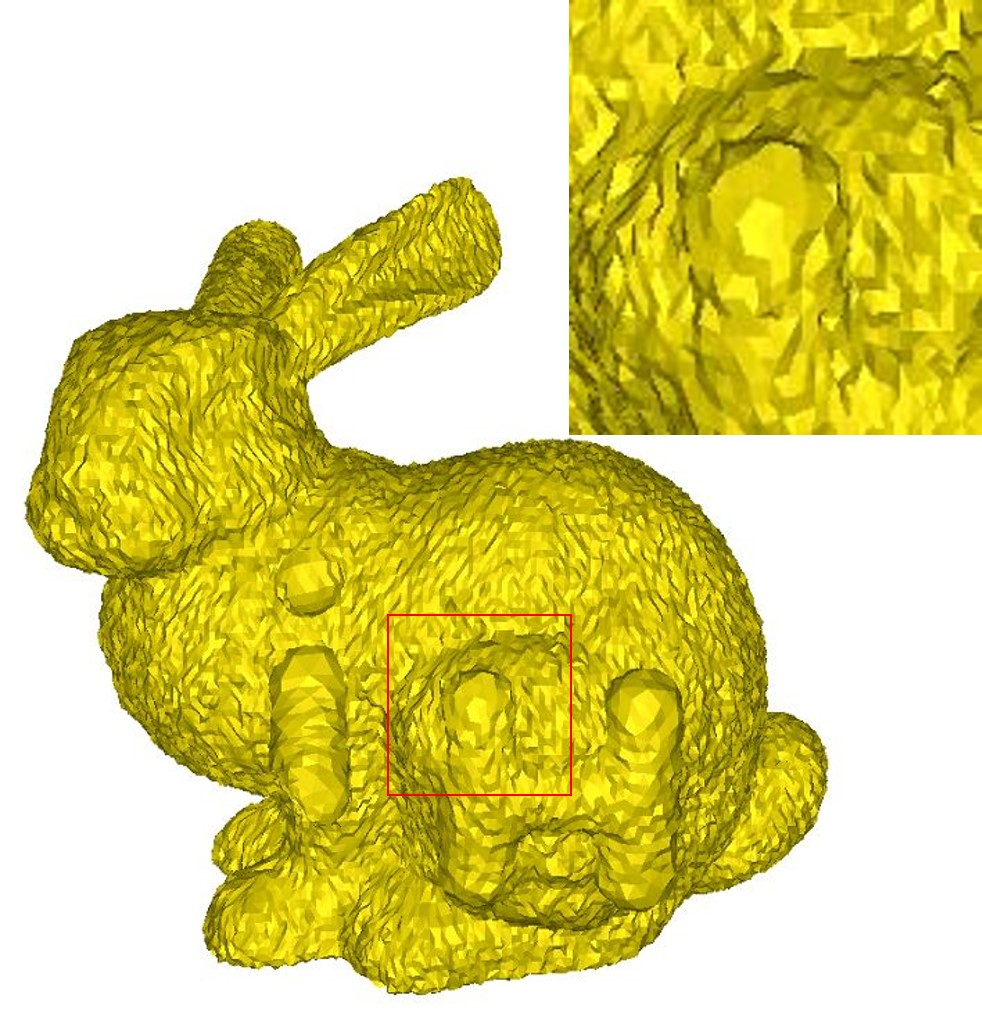
\includegraphics[width = 1.8cm]{results/Bunny0.2/snapshot00C.jpg}}
\subfigure
{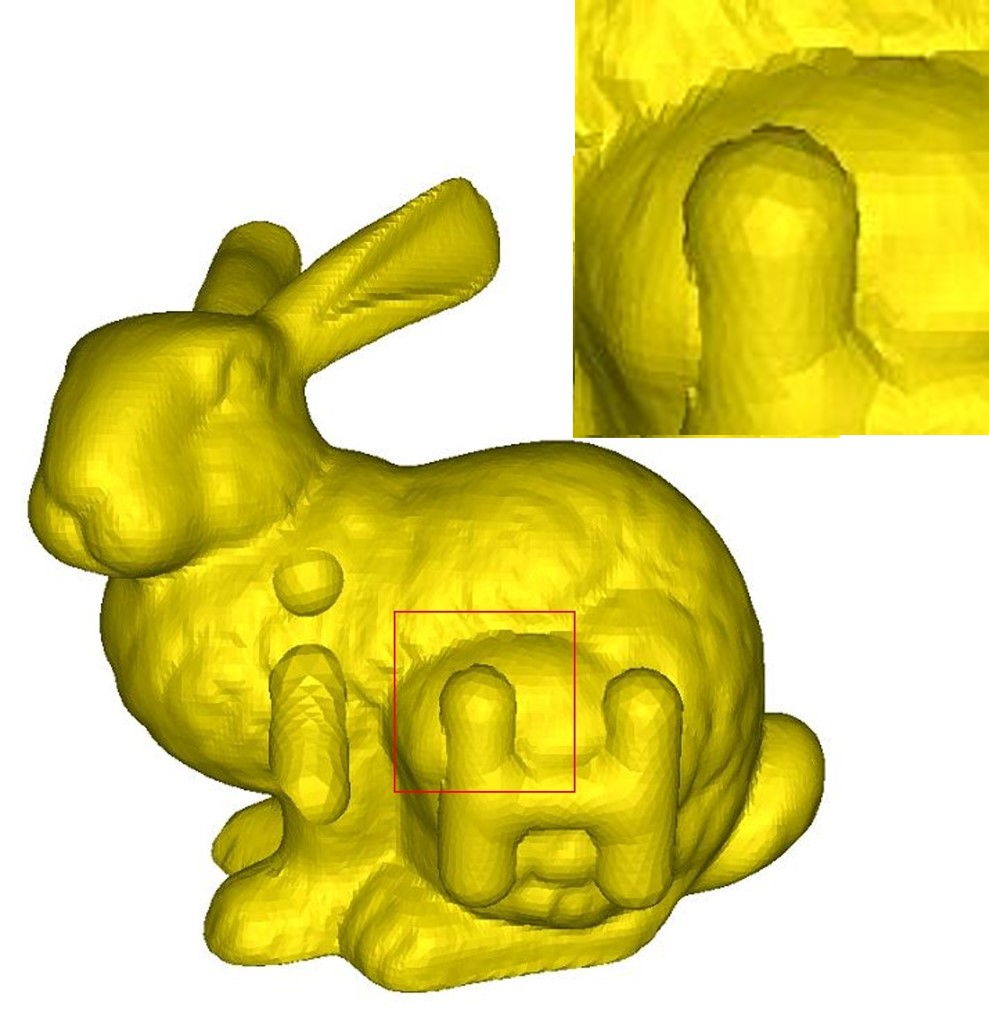
\includegraphics[width = 1.8cm]{results/Bunny0.2/snapshot01C.jpg}}
\subfigure
{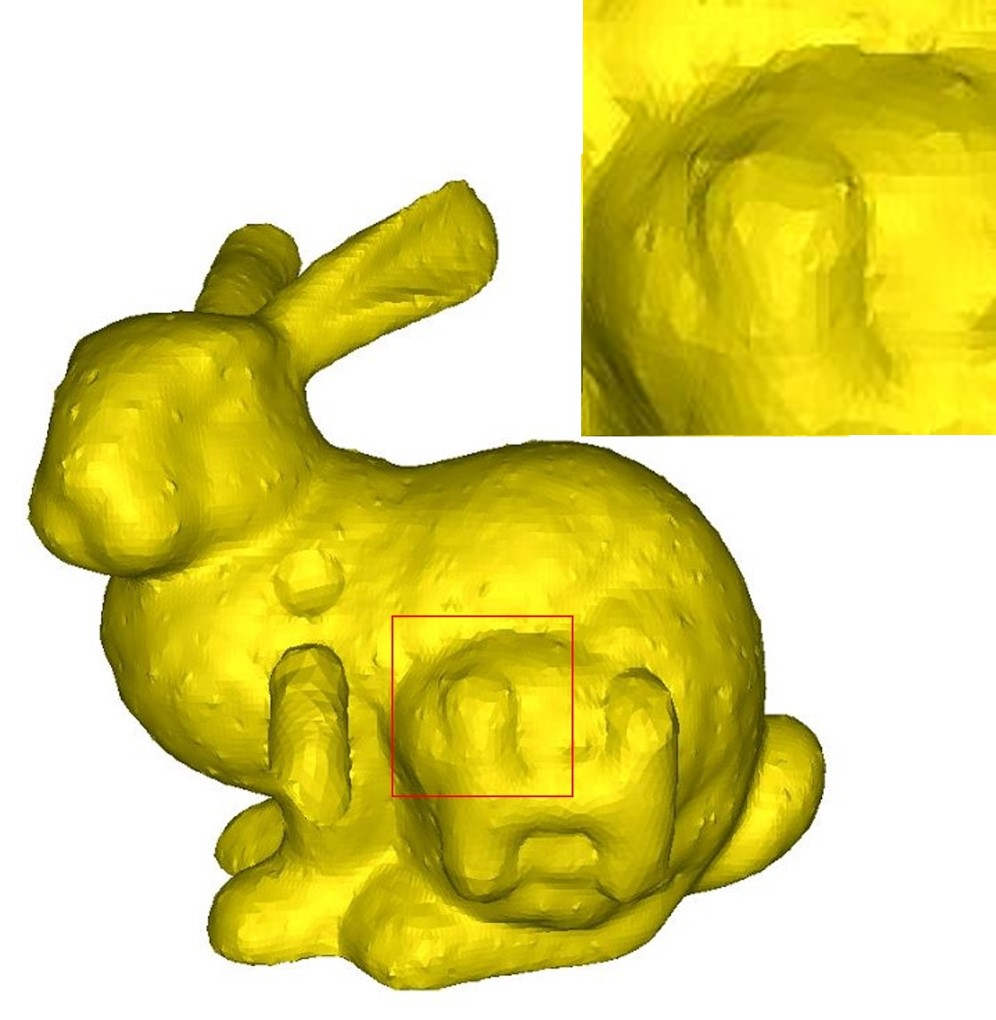
\includegraphics[width = 1.8cm]{results/Bunny0.2/snapshot02C.jpg}}
\subfigure
{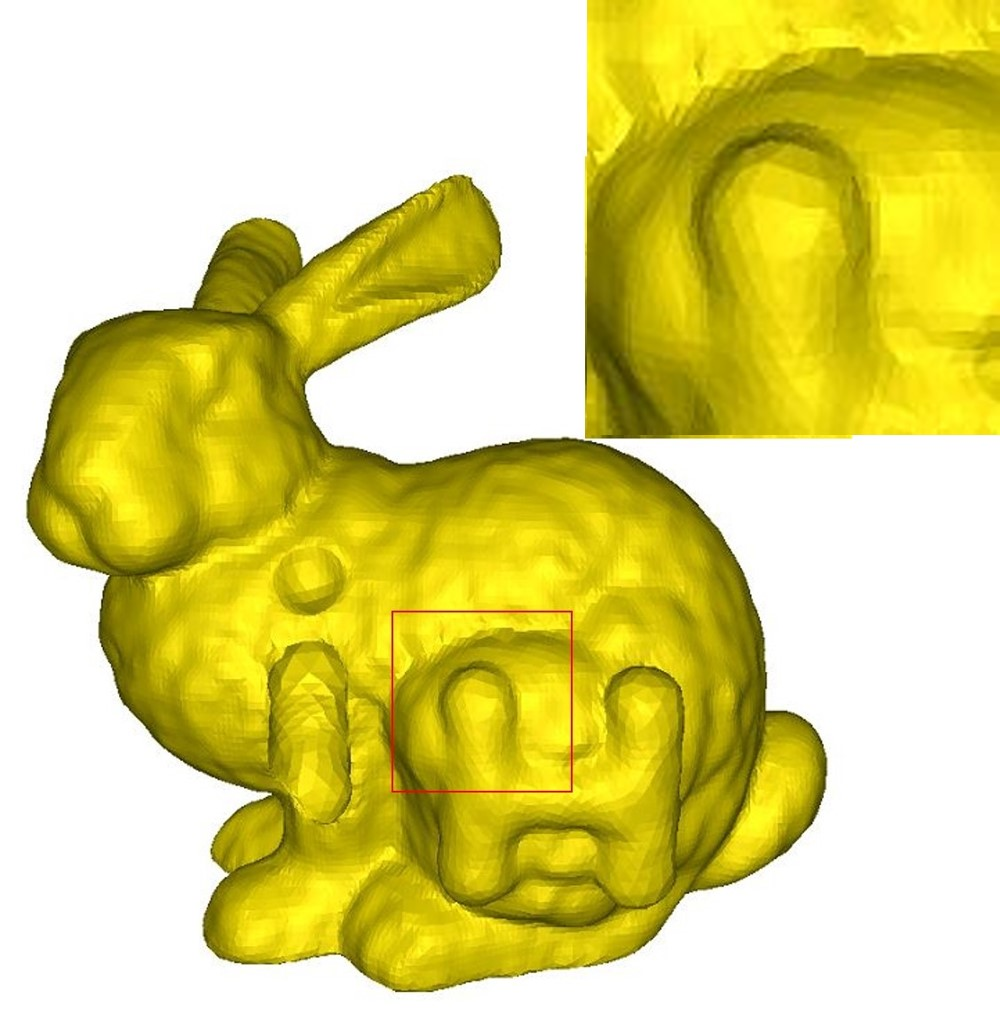
\includegraphics[width = 1.8cm]{results/Bunny0.2/snapshot03C.jpg}}
\subfigure
{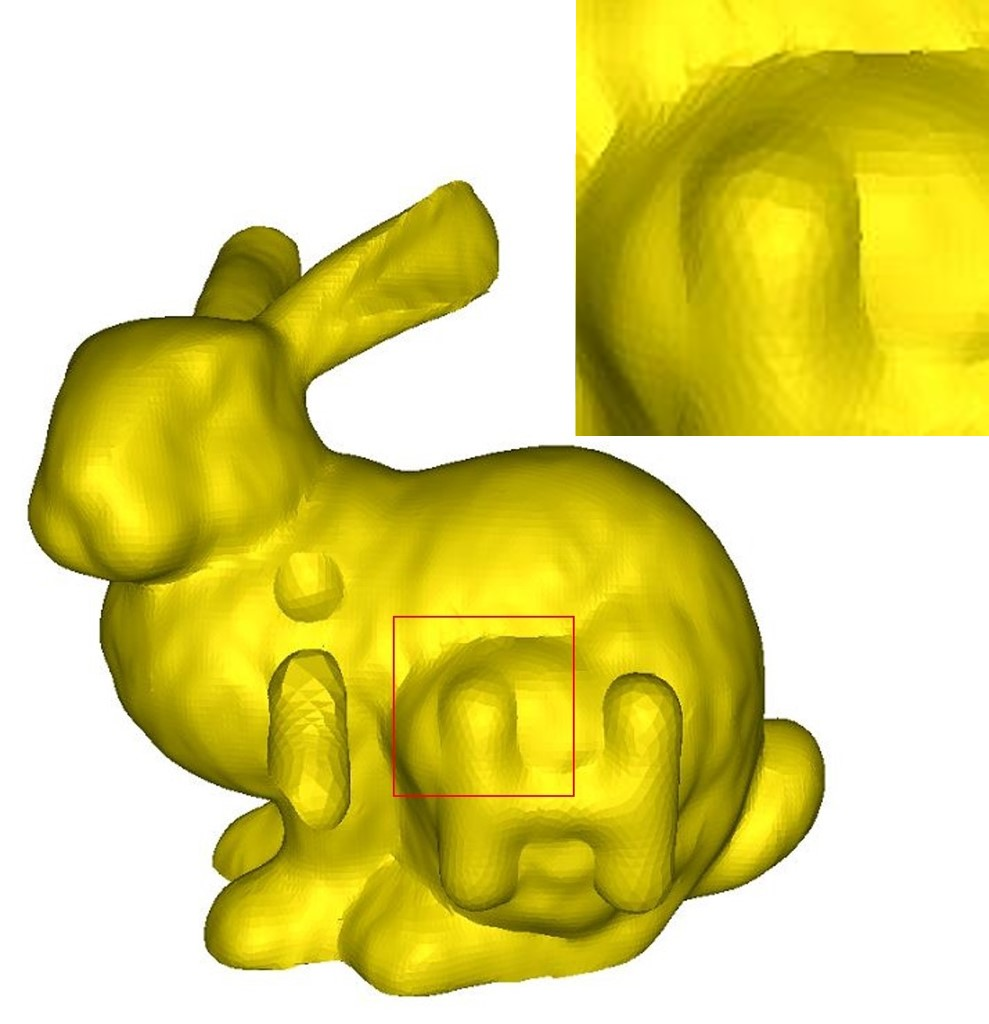
\includegraphics[width = 1.8cm]{results/Bunny0.2/snapshot04C.jpg}}
\subfigure
{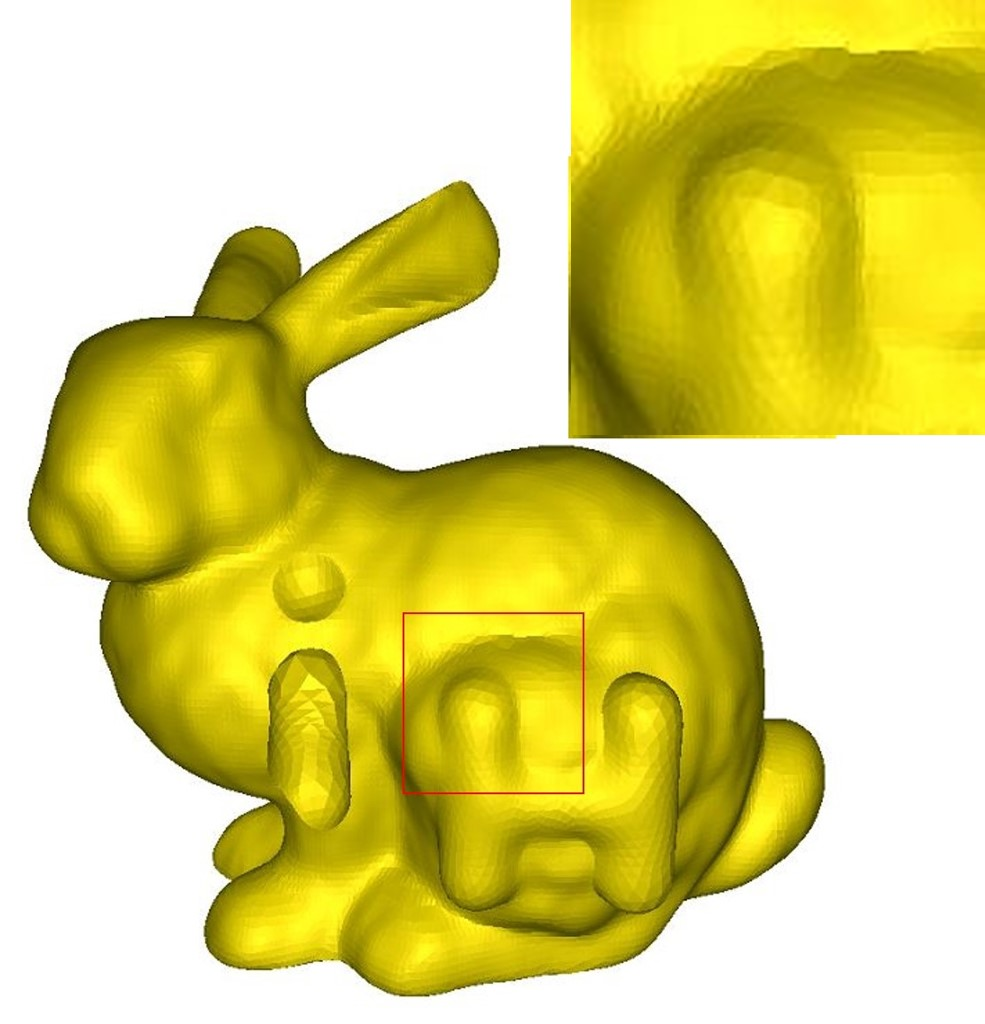
\includegraphics[width = 1.8cm]{results/Bunny0.2/snapshot05C.jpg}}
\subfigure
{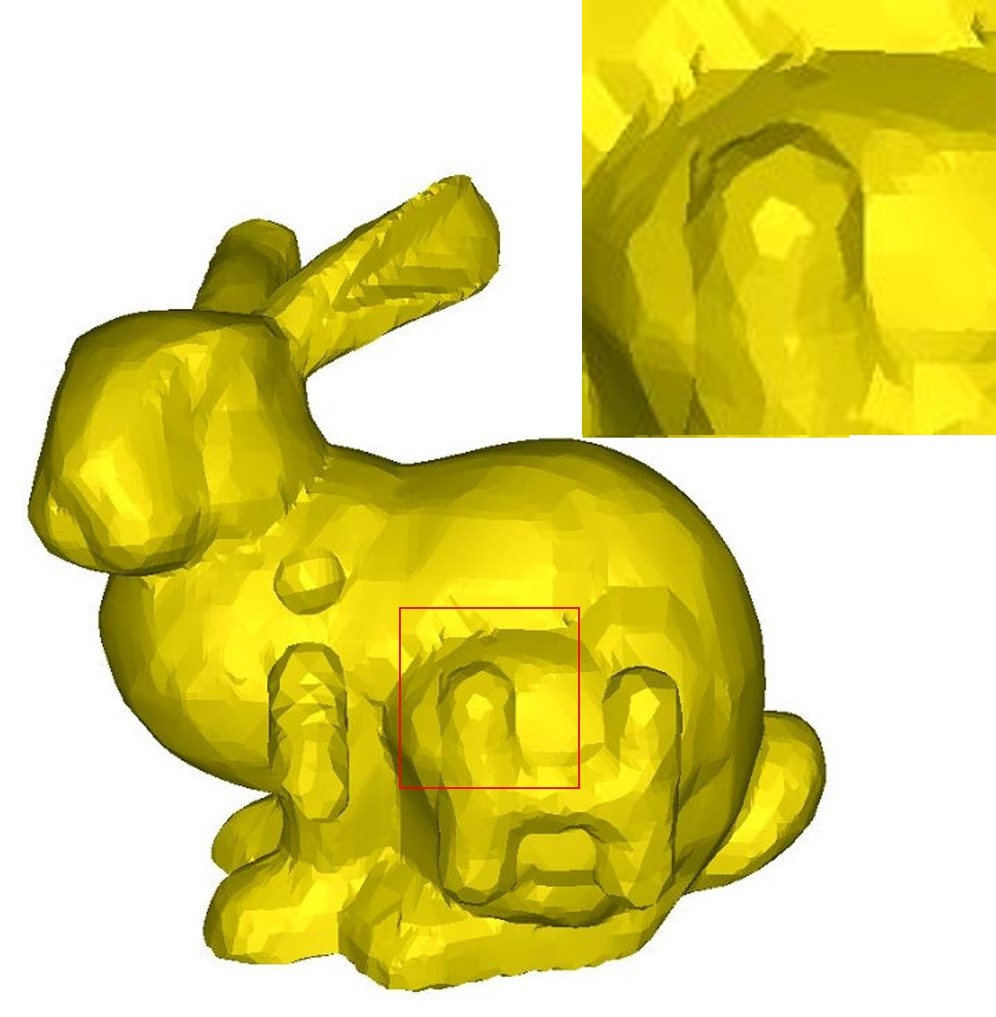
\includegraphics[width = 1.8cm]{results/Bunny0.2/snapshot06C.jpg}}
\subfigure
{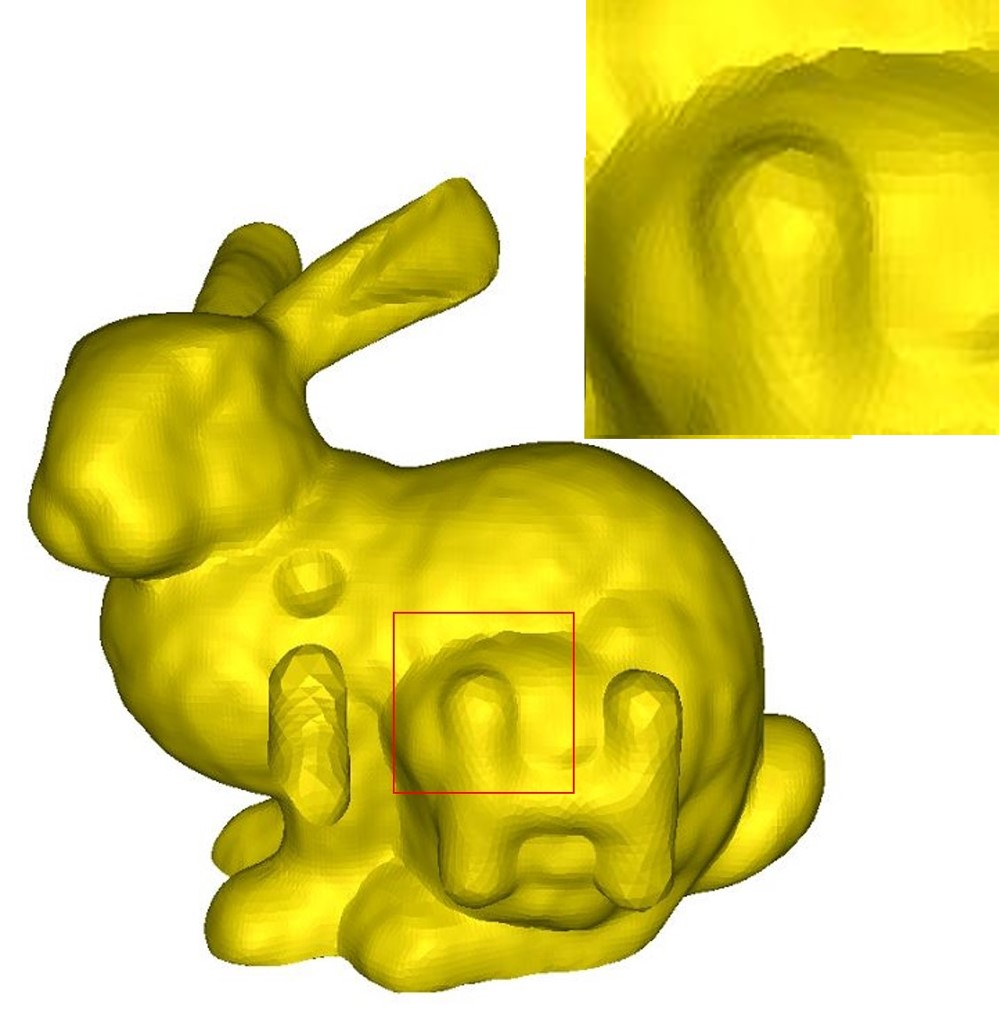
\includegraphics[width = 1.8cm]{results/Bunny0.2/snapshot07C.jpg}}
\subfigure
{\includegraphics[width = 1.8cm]{results/Bunny0.2/snapshot08C.jpg}}
\\
\vspace{-1.2mm}

\subfigure
{\includegraphics[width = 1.8cm]{results/Julius0.2/snapshot00.jpg}}
\subfigure
{\includegraphics[width = 1.8cm]{results/Julius0.2/snapshot01.jpg}}
\subfigure
{\includegraphics[width = 1.8cm]{results/Julius0.2/snapshot02.jpg}}
\subfigure
{\includegraphics[width = 1.8cm]{results/Julius0.2/snapshot03.jpg}}
\subfigure
{\includegraphics[width = 1.8cm]{results/Julius0.2/snapshot04.jpg}}
\subfigure
{\includegraphics[width = 1.8cm]{results/Julius0.2/snapshot05.jpg}}
\subfigure
{\includegraphics[width = 1.8cm]{results/Julius0.2/snapshot06.jpg}}
\subfigure
{\includegraphics[width = 1.8cm]{results/Julius0.2/snapshot07.jpg}}
\subfigure
{\includegraphics[width = 1.8cm]{results/Julius0.2/snapshot08.jpg}}
\caption{ Comparisons with other methods on synthetic meshes with additive Gaussian noise.
The results are from left to right noisy mesh, original mesh, \cite{fleishman2003bilateral}, \cite{jones2003non}, \cite{sun2007fast},
\cite{zheng2011bilateral}, \cite{he2013mesh}, \cite{Zhang2015Filter} and ours respectively.
The intensity $\sigma_E$ of the noise is from the top to bottom 0.3, 0.1, 0.2 and 0.2.}
\label{Fig:datasets}
\end{figure*}


{\bfseries Comparison with other methods on the synthetic meshes.}

Figure~\ref{Fig:octahedron} witnesses the effectiveness of our model on non-uniform sampling mesh.
Note that we make subdivision on a strong edge and a sharp corner of the octahedron model.
These regions are shown in the red rectangle boxes and one that not do subdivision is used for comparison.
From the results, the approaches of ~\cite{fleishman2003bilateral, jones2003non} can not well deal with the strong edges, because the spatial weight weaken the strength of filtering.
Although~\cite{sun2007fast, zheng2011bilateral, he2013mesh} have the ability to maintain the mesh strong edge structure, they lose the effectiveness in the non-uniform sampling regions.
The reason is that these region have larger normal difference than others, so these algorithms are hard to weight the two aspects.
While~\cite{Zhang2015Filter} can well maintain the strong edge structure of mesh and also deal with non-uniform sampling problem.
However, as the local structure of sharp corner is special, the guided normal of~\cite{Zhang2015Filter} may be prone to ambiguity.
Hence, \cite{Zhang2015Filter} do not well deal with the sharp corners.
Our model do well in these conditions
not only our weight design by two kinds of accumulative normal differences
but also the function of six regions which give a better estimation in the structure of local mesh.


Our algorithm obtains satisfactory results in mesh denoising shown in the figure~\ref{Fig:datasets}.
This figure contains four models, respectively is fandisk, prism, bunny and Julius.
Our method and~\cite{Zhang2015Filter} both have the power on preserving the mesh weak feature than others~\cite{fleishman2003bilateral, jones2003non, sun2007fast, zheng2011bilateral, he2013mesh}
from the fandisk model, but \cite{Zhang2015Filter} still hardly maintains the sharp corners in fandisk model.
The prism with 18 edges is used for explain the ability in dealing with the same strength weak feature among these methods.
After removing most noises, \cite{fleishman2003bilateral, jones2003non, sun2007fast, zheng2011bilateral} can not restore the edge structure of prism.
\cite{he2013mesh, Zhang2015Filter} can recover the original structure, but they damage the straight line feature of prism.
However, our method can well retains the mesh structures from the above two models.
Bunny and Julius models also show us that our method can preserve the mesh detail while smoothing the noise.


Table~\ref{Tab:1} shows the quantitative errors according to the two equations~\ref{Eq:vertexerror} and~\ref{Eq:normalerror}.
For most of the models, our method achieves better results than others.
In general, we demonstrate that our model can compare with the state-of-the-art methods.
The detail of our and their parameters can be found in the supplementary material.

%In the figure~\ref{Fig:special}, we show our method also can deal with different kinds of noise.
%From the vision, our method almost obtains the similar results comparing with Zhang et al~\cite{Zhang2015Filter}.
%However, according to the table~\ref{Tab:1}, our method works well.

\begin{table*}[ht]
\caption{Quantitative comparisons using two error metrics. For each model, the best error metric value is highlighted.}
\vspace{2mm}
\label{Tab:1}
\begin{center}
\begin{tabular}{|c|c|c|c|c|c|c|c|c|} %% this creates eight columns also can be "c" and "r", "|" representative inserting ����
%% |l|l| to left justify each column entry
%% |c|c| to center each column entry
%% use of \rule[]{}{} below opens up each row
\hline
\rule[-1ex]{0pt}{3.5ex}  Model & Error  &  \cite{fleishman2003bilateral}  & \cite{jones2003non} & \cite{sun2007fast} & \cite{zheng2011bilateral} & \cite{he2013mesh} & \cite{Zhang2015Filter} & ours \\
\hline\hline

\rule[-1ex]{0pt}{3.5ex}  \multirow{2}{*}{Octahedron (Fig~\ref{Fig:octahedron})}
& \jj{$E_n$} & 12.81 & 10.65 & 6.85 & 5.27 & 3.33 & 3.36 & \textbf{1.00} \\
\cline{2-9}
& \jj{$E_v(\times10^{-3})$} & 28.02 & 14.70 & 10.71 & 6.28 & 10.81 & 4.90 & \textbf{3.02}\\
\hline

\rule[-1ex]{0pt}{3.5ex}  \multirow{2}{*}{Fandisk (Fig~\ref{Fig:datasets})}
& $E_n$ & 9.73 & 9.82 & 4.04 & 3.35 & 5.53 & 2.62 & \textbf{2.27} \\
\cline{2-9}
& $E_v(\times10^{-3})$ & 18.14 & 15.10 & 11.02 & 8.72 & 18.79 & \textbf{6.29} & 6.35\\
\hline

\rule[-1ex]{0pt}{3.5ex}  \multirow{2}{*}{Prism (Fig~\ref{Fig:datasets})}
& $E_n$ & 4.98 & 4.48 & 3.29 & 3.87 & 0.71 & 0.87 & \textbf{0.46} \\
\cline{2-9}
& $E_v(\times10^{-2})$ & 11.89 & 10.46 & 7.45 & 7.9  & 3.42 & 4.09 & \textbf{2.77}\\
\hline

%\rule[-1ex]{0pt}{3.5ex}  \multirow{2}{*}{sphere (Fig~\ref{Fig:datasets})}
%& $E_n$ & 12.58 & 17.36 & 11.89 & \textbf{6.70} & 12.96 & 10.17 & 7.39 \\
%\cline{2-9}
%& $E_v(\times10^{-2})$ & 15.51 & 8.46 & 8.88 & 4.48 & 12.41 & 5.65 & \textbf{4.37}\\
%\hline

\rule[-1ex]{0pt}{3.5ex}  \multirow{2}{*}{Bunny (Fig~\ref{Fig:datasets})}
& $E_n$ & 6.93 & 5.81 & 5.89 & 5.68 & 7.21 & 5.35 & \textbf{5.11} \\
\cline{2-9}
& $E_v(\times10^{-4})$ & 18.36 & 9.24 & 9.98 & 9.35 & 10.65 & 7.61 & \textbf{7.26}\\
\hline

\rule[-1ex]{0pt}{3.5ex}  \multirow{2}{*}{Julius (Fig~\ref{Fig:datasets})}
& $E_n$ & 7.70 & 7.63 & 7.01 & 6.21 & 7.98 & 6.38 & \textbf{6.11} \\
\cline{2-9}
& $E_v(\times10^{-4})$ & 10.58 & 7.71 & 6.49 & \textbf{5.53} & 8.60 & 6.02 & 5.78\\
\hline

%\rule[-1ex]{0pt}{3.5ex}  \multirow{2}{*}{block (Fig~\ref{Fig:special})}
%& $E_n$ & 12.72 & 13.85 & 5.80 & 5.31 & 4.97 & 3.57 & \textbf{3.02} \\
%\cline{2-9}
%& $E_v(\times10^{-2})$ & 17.98 & 13.35 & 8.21 & 6.80 & 11.60 & 5.41 & \textbf{4.99}\\
%\hline

%\rule[-1ex]{0pt}{3.5ex}  \multirow{2}{*}{twelve (Fig~\ref{Fig:special})}
%& $E_n$ & 11.72 & 11.09 & 7.45 & 7.37 & 8.46 & 2.75 & \textbf{1.78} \\
%\cline{2-9}
%& $E_v(\times10^{-3})$ & 20.85 & 17.28 & 12.06 & 12.54  & 20.13 & 6.16 & \textbf{5.23}\\
%\hline

%\rule[-1ex]{0pt}{3.5ex}  \multirow{2}{*}{Nicolo}
%& $E_n$ & 8.88 & 7.13 & 6.38 & \textbf{5.80} & 7.58 & 6.50 & 5.93 \\
%\cline{2-9}
%& $E_v(\times10^{-1})$ & 4.60 & 3.33 & 3.18 & 2.59  & 3.48 & 2.61 & \textbf{2.50}\\
%\hline

\end{tabular}
\end{center}
\end{table*}


{\bfseries Comparison with other methods on the real noisy meshes.}

We also test our algorithm on the real-world 3d models with the above methods and further demonstrate the effectiveness of our model.
Figure~\ref{Fig:TrueMesh} illustrates the three real scanned models, angel, rabbit and iron respectively.
From the eye of angel, our model depicts the eyelid well.
And the iron model also reveals the ability in maintaining the edge structure. 

Table~\ref{Tab:Time} provides the timing of our approach for the shown examples, on a PC with an Intel Core $i7-4790K$.
Even with those bigger mesh, the time of our algorithm is acceptable.

\begin{figure*}[htb]
\centering

\subfigure
{\includegraphics[width = 2.0cm]{results/Angel/snapshot00C.jpg}}
\subfigure
{\includegraphics[width = 2.0cm]{results/Angel/snapshot01C.jpg}}
\subfigure
{\includegraphics[width = 2.0cm]{results/Angel/snapshot02C.jpg}}
\subfigure
{\includegraphics[width = 2.0cm]{results/Angel/snapshot03C.jpg}}
\subfigure
{\includegraphics[width = 2.0cm]{results/Angel/snapshot04C.jpg}}
\subfigure
{\includegraphics[width = 2.0cm]{results/Angel/snapshot05C.jpg}}
\subfigure
{\includegraphics[width = 2.0cm]{results/Angel/snapshot06C.jpg}}
\subfigure
{\includegraphics[width = 2.0cm]{results/Angel/snapshot07C.jpg}}
\\
\vspace{-2.0mm}
\subfigure
{\includegraphics[width = 2.0cm]{results/Rabbit/snapshot00.jpg}}
\subfigure
{\includegraphics[width = 2.0cm]{results/Rabbit/snapshot01.jpg}}
\subfigure
{\includegraphics[width = 2.0cm]{results/Rabbit/snapshot02.jpg}}
\subfigure
{\includegraphics[width = 2.0cm]{results/Rabbit/snapshot03.jpg}}
\subfigure
{\includegraphics[width = 2.0cm]{results/Rabbit/snapshot04.jpg}}
\subfigure
{\includegraphics[width = 2.0cm]{results/Rabbit/snapshot05.jpg}}
\subfigure
{\includegraphics[width = 2.0cm]{results/Rabbit/snapshot06.jpg}}
\subfigure
{\includegraphics[width = 2.0cm]{results/Rabbit/snapshot07.jpg}}
\\
\vspace{-2.0mm}
\subfigure
{\includegraphics[width = 2.0cm]{results/Iron/snapshot00C.jpg}}
\subfigure
{\includegraphics[width = 2.0cm]{results/Iron/snapshot01C.jpg}}
\subfigure
{\includegraphics[width = 2.0cm]{results/Iron/snapshot02C.jpg}}
\subfigure
{\includegraphics[width = 2.0cm]{results/Iron/snapshot03C.jpg}}
\subfigure
{\includegraphics[width = 2.0cm]{results/Iron/snapshot04C.jpg}}
\subfigure
{\includegraphics[width = 2.0cm]{results/Iron/snapshot05C.jpg}}
\subfigure
{\includegraphics[width = 2.0cm]{results/Iron/snapshot06C.jpg}}
\subfigure
{\includegraphics[width = 2.0cm]{results/Iron/snapshot07C.jpg}}
\vspace{0.5mm}
\caption{ The real noisy mesh. The results are from left to right noisy mesh, original mesh
, \cite{fleishman2003bilateral}, \cite{jones2003non}, \cite{sun2007fast}, \cite{zheng2011bilateral}(l), \cite{he2013mesh}, \cite{Zhang2015Filter} and ours respectively.}
\label{Fig:TrueMesh}
\end{figure*}

\begin{table}[htb]
\caption{Time consumption for different results. }
\vspace{2mm}
\label{Tab:Time}
\begin{center}
\begin{tabular}{|c|c|c|c|c|}
\hline
\rule[-1ex]{0pt}{3.5ex} Model & Vertics & Faces & Time(s) & $k_{iter}$ \\
\hline\hline

\rule[-1ex]{0pt}{3.5ex} Octahedron (Fig~\ref{Fig:octahedron}) & Vertices & Faces & Time(s) & $k_{iter}$ \\
\hline

\rule[-1ex]{0pt}{3.5ex} Fandisk (Fig~\ref{Fig:datasets}) & 6475 & 12946 & 2.77 & 30 \\
\hline

\rule[-1ex]{0pt}{3.5ex} Prism (Fig~\ref{Fig:datasets}) & Vertices & Faces & Time(s) & $k_{iter}$ \\
\hline

\rule[-1ex]{0pt}{3.5ex} Bunny (Fig~\ref{Fig:datasets}) & 34834 & 69451 & 4.33 & 4 \\
\hline

\rule[-1ex]{0pt}{3.5ex} Julius (Fig~\ref{Fig:datasets}) & 36201 & 71912 & 3.54 & 4 \\
\hline
%\rule[-1ex]{0pt}{3.5ex} Twelve (Fig~\ref{Fig:Impulsive}) & 4610 & 9216 & 7.03 & 50 \\
%\hline

\rule[-1ex]{0pt}{3.5ex} Angel (Fig~\ref{Fig:TrueMesh}) & 24566 & 48090 &  & $k_{iter}$ \\
\hline

\rule[-1ex]{0pt}{3.5ex} Rabbit (Fig~\ref{Fig:TrueMesh}) & 37394 & 73679 &  & $k_{iter}$ \\
\hline

\rule[-1ex]{0pt}{3.5ex} Iron (Fig~\ref{Fig:TrueMesh}) & 85574 & 168285 &  & $k_{iter}$ \\
\hline

\end{tabular}
\end{center}
\end{table}

\subsection{Limitation and discussion}

Although our model is effective for denoising most meshes, it still has some limitations.
First, although we control the normal difference by $\sigma_r$ and $\sigma_s$, our parameters can not adaptively change according the local characteristic of mesh, inevitably lost some details.
Second, our algorithm easily generates folded triangles in some cases.
The process of vertex update may results in the error, because it only depends on the orthogonality between the filtered normals and the new edges.
Third, our algorithm can not guarantee algorithm convergence from the figure~\ref{Fig:Convergence}.
The main reason is that we apply local strategy to filter face normals, which not ensures the global structure of mesh.
For solving this problem, we need use a global filtering strategy like~\cite{zheng2011bilateral}.
\begin{figure}[htb]
\centering
\includegraphics[width = 8cm]{results/convergence.jpg}
\vspace{0.5mm}
\caption{ the convergence.\jj{(figure should be changed)}}
\label{Fig:Convergence}
\end{figure}

\section{Conclusion}

In this paper, we introduce a intrinsic signal filtering framework for denoising 2D manifold surface.
Intrinsically, our method builds the relation between desired filtering signals and its neighbors, making calculate weights more reasonably.
Other famous filtering algorithm, such as bilateral, geodesic and propagation filters, can be simplified by our algorithm.
Furthermore, we apply our filtering framework to triangular meshes and obtain state-of-the-art performance.
We also propose a simple, fast and effective method for choosing path in the process of intrinsic filtering algorithm instead of geodesic path.
And, the approach for dividing region protects the local mesh structure in a certain extent, further increasing the effectiveness of mesh filter.
Finally, a large number of experiments prove the effectiveness of our method.




{\bfseries Acknowledgements}

%\input{conclusion}

%\section*{Acknowledgements}
%Do not forget.
%-------------------------------------------------------------------------

{\small
\bibliographystyle{cvm}
\bibliography{PropagatedDenoising}
}


\end{document}
